% !TeX root = ../../report.tex
\section{Timer Interrupt and LED Scanning}

\subsection{Introduction}
Timers are one of the most important features in modern micro-controllers. They allow us to measure how long something takes to execute, create non-blocking code, precisely control pin timing, and even run operating systems. In this manual, how to configure a timer using STM32CubeIDE is presented how to use them to flash an LED. Finally, students are proposed to finalize 10 exercises using timer interrupt for applications based LED Scanning.

\begin{figure}[!htp]
    \centering
    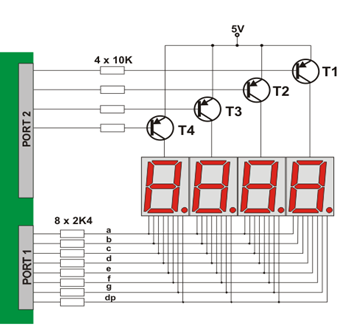
\includegraphics[width=3.5in]{source/picture/bai_2/led_scanning1.png}
    \caption{\textit{Four seven segment LED interface for a micro-controller}}
    \label{bai2_intro1}
\end{figure}


Design an interface for with multiple LED (seven segment or matrix) displays which is to be controlled is depends on the number of input and output pins needed for controlling all the LEDs in the given matrix display, the amount of current that each pin can source and sink and the speed at which the micro-controller can send out control signals. With all these specifications, interfacing can be done for 4 seven segment LEDs with a micro-controller is proposed in the figure above. \\


In the above diagram each seven segment display is having 8 internal LEDs, leading to the total number of LEDs is 32. However, not all the LEDs are required to turn ON, but one of them is needed. Therefore, only 12 lines are needed to control the whole 4 seven segment LEDs.   By controlling with the micro-controller, we can turn ON an LED during a same interval \textbf{$T_S$}. Therfore, the period for controlling all 4 seven segment LEDs is \textbf{$4T_S$}. In other words, these LEDs are scanned at frequecy \textbf{$f = 1 / 4T_S$}. Finally, it is obviously that if the frequency is greater than 30Hz (e.g. f = 50Hz), it seems that all LEDs are turn ON at the same time.\\

In this manual, the timer interrupt is used to design the interval $T_S$ for LED scanning. Unfortunately, the simulation on Proteus can not execute at high frequency, the frequency $f$ is set to a low value (e.g. 1Hz). In a real implementation, this frequency should be 50Hz.


\newpage
\subsection{Timer Interrupt Setup}
\textbf{Step 1: } Create a simple project, which LED connected to PA5. The manual can be found in the first lab.\\

\textbf{Step 2: } Check the clock source of the system on the tab \textbf{Clock Configuration} (from *.ioc file). In the default configuration, the internal clock source is used with 8MHz, as shown in the figure bellow.

\begin{figure}[!htp]
    \centering
    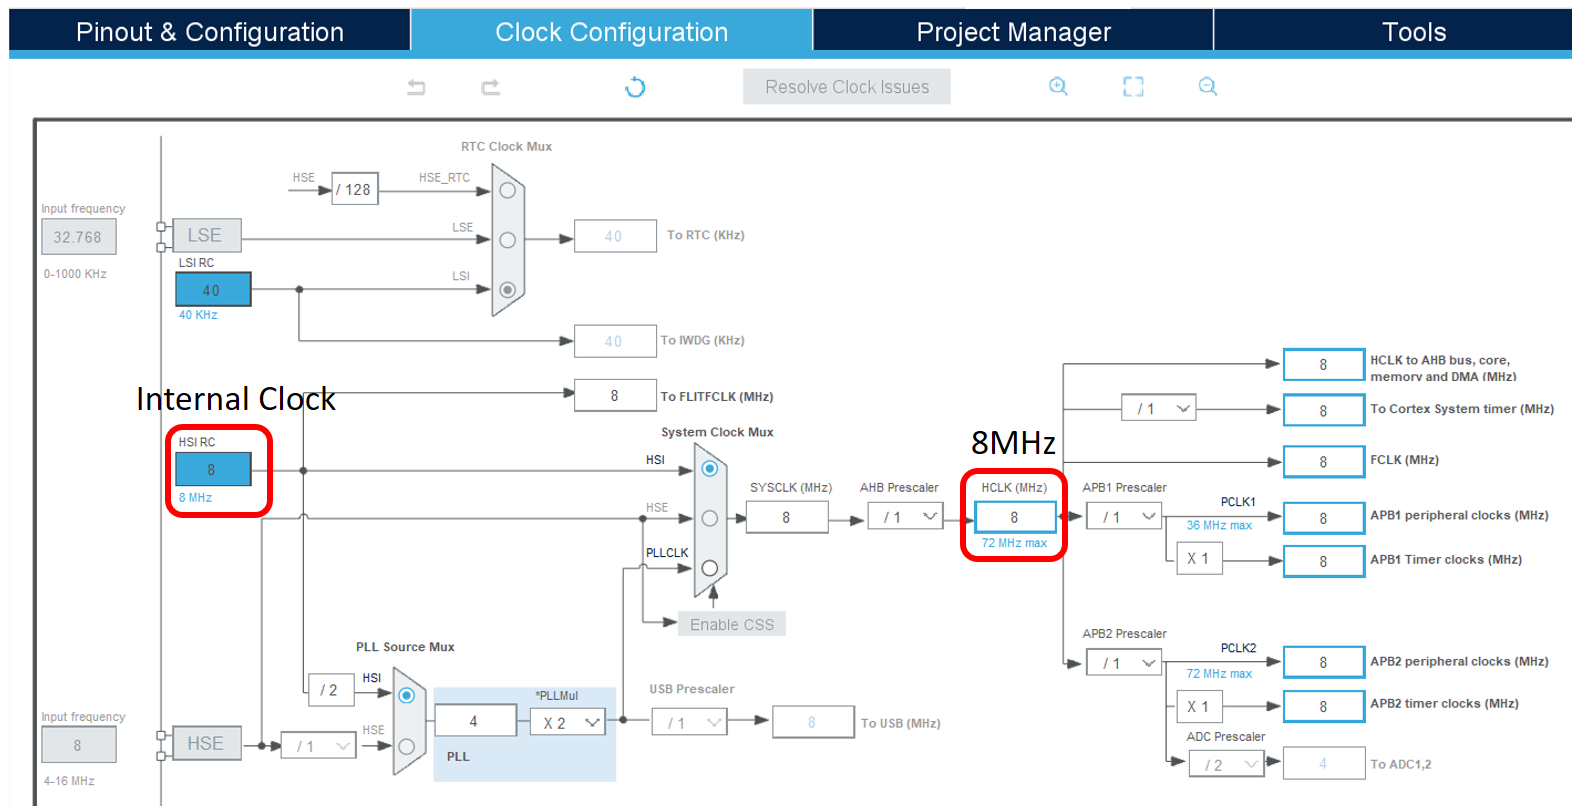
\includegraphics[width=5.5in]{source/picture/bai_2/lab2_m1.PNG}
    \caption{\textit{Default clock source for the system}}
    \label{bai2_m1}
\end{figure}

\textbf{Step 3: } Configure the timer on the \textbf{Parameter Settings}, as follows:
\begin{figure}[!htp]
    \centering
    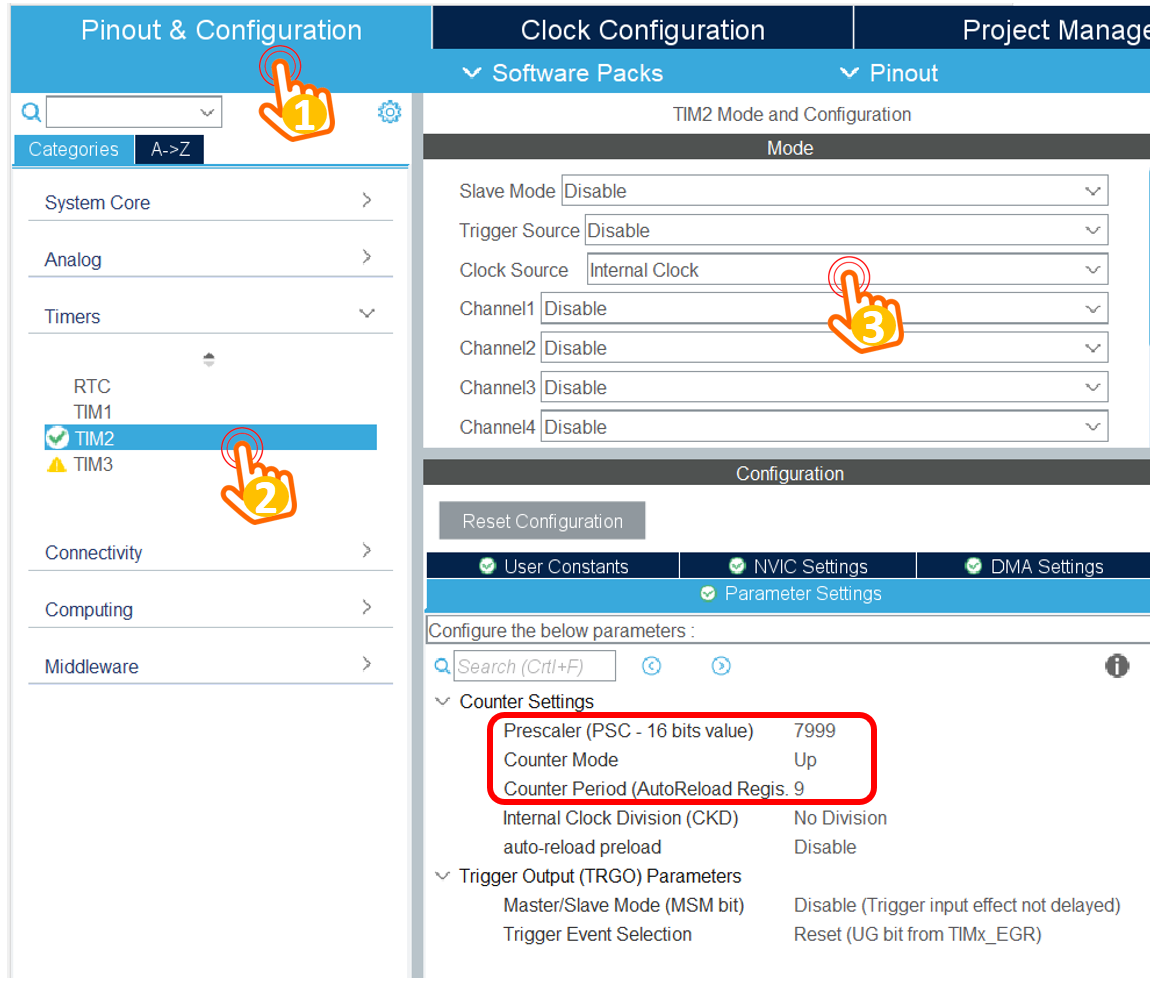
\includegraphics[width=3.5in]{source/picture/bai_2/lab2_m2.PNG}
    \caption{\textit{Configure for Timer 2}}
    \label{bai2_m2}
\end{figure}

Select the clock source for timer 2 to the \textbf{Internal Clock}. Finally, set the prescaller and the counter to 7999 and 9, respectively. These values are explained as follows:
\begin{itemize}
    \item The target is to set an interrupt timer to 10ms
    \item The clock source is 8MHz, by setting the prescaller to 7999, the input clock source to the timer is \textbf{8MHz/(7999+1) = 1000Hz}.
    \item The interrupt is raised when the timer counter is counted from 0 to 9, meaning that the frequency is divided by 10, which is 100Hz.
    \item The frequency of the timer interrupt is 100Hz, meaning that the period is \textbf{1/100Hz = 10ms}.
\end{itemize}

\textbf{Step 4: } Enable the timer interrupt by switching to \textbf{NIVC Settings} tab, as follows:

\begin{figure}[!htp]
    \centering
    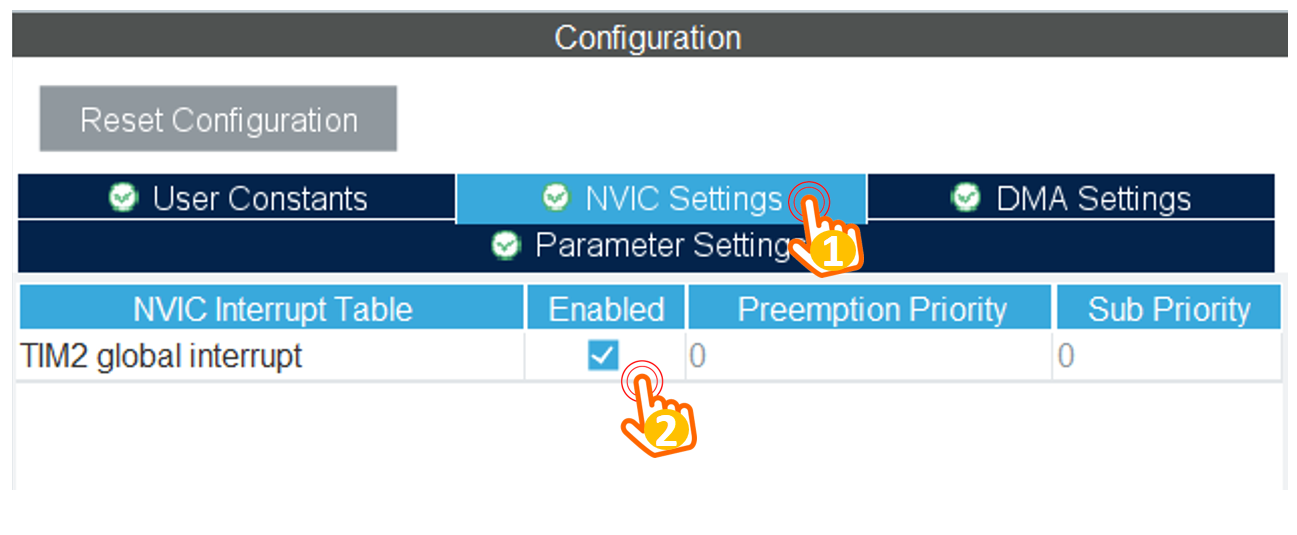
\includegraphics[width=4in]{source/picture/bai_2/lab2_m3.PNG}
    \caption{\textit{Enable timer interrupt}}
    \label{bai2_m3}
\end{figure}

Finally, save the configuration file to generate the source code.\\

\textbf{Step 5: } On the \textbf{main()} function, call the timer init function, as follows:

\begin{lstlisting}[caption=Init the timer interrupt in main]
int main(void)
{
  HAL_Init();
  SystemClock_Config();

  MX_GPIO_Init();
  MX_TIM2_Init();
  
  /* USER CODE BEGIN 2 */
  HAL_TIM_Base_Start_IT(&htim2);
  /* USER CODE END 2 */

  while (1){
  
  }
}
\end{lstlisting}

Please put the init function in a right place to avoid conflicts when code generation is executed (e.g. ioc file is updated).\\
\newpage
\textbf{Step 6: } Add the interrupt service routine function, this function is invoked every 10ms, as follows:

\begin{lstlisting}[caption=Add an interrupt service routine]
/* USER CODE BEGIN 4 */
void HAL_TIM_PeriodElapsedCallback(TIM_HandleTypeDef *htim){
	
}
/* USER CODE END 4 */
\end{lstlisting}

\textbf{Step 7: } To run a LED Blinky demo using interrupt, a short manual is presented as follows:
\begin{lstlisting}[caption=LED Blinky using timer interrupt]
/* USER CODE BEGIN 4 */
int counter = 100;
void HAL_TIM_PeriodElapsedCallback(TIM_HandleTypeDef *htim){
	counter--;
	if(counter <= 0){
		counter = 100;
		HAL_GPIO_TogglePin(LED_RED_GPIO_Port, LED_RED_Pin);
	}
}
/* USER CODE END 4 */
\end{lstlisting}

The \textbf{HAL\_TIM\_PeriodElapsedCallback} function is an infinite loop, which is invoked every cycle of the timer 2, in this case, is 10ms.\\



\newpage
\subsection{Exercise and Report}
\subsubsection{Exercise 1}
The first exercise show how to interface for multiple seven segment LEDs to STM32F103C6 micro-controller (MCU). Seven segment displays are common anode type, meaning that the anode of all LEDs are tied together as a single terminal and cathodes are left alone as individual pins. \\

In order to save the resource of the MCU, individual cathode pins from all the seven segment LEDs are connected together, and connect to 7 pins of the MCU. These pins are popular known as the \textbf{signal pins}. Meanwhile, the anode pin of each seven segment LEDs are controlled under a power enabling circuit, for instance, an PNP transistor. At a given time, only one seven segment LED is turned on. However, if the delay is small enough, it seems that all LEDs are enabling. \\

Implement the circuit simulation in Proteus with two 7-SEGMENT LEDs as following:

\begin{figure}[!htp]
    \centering
    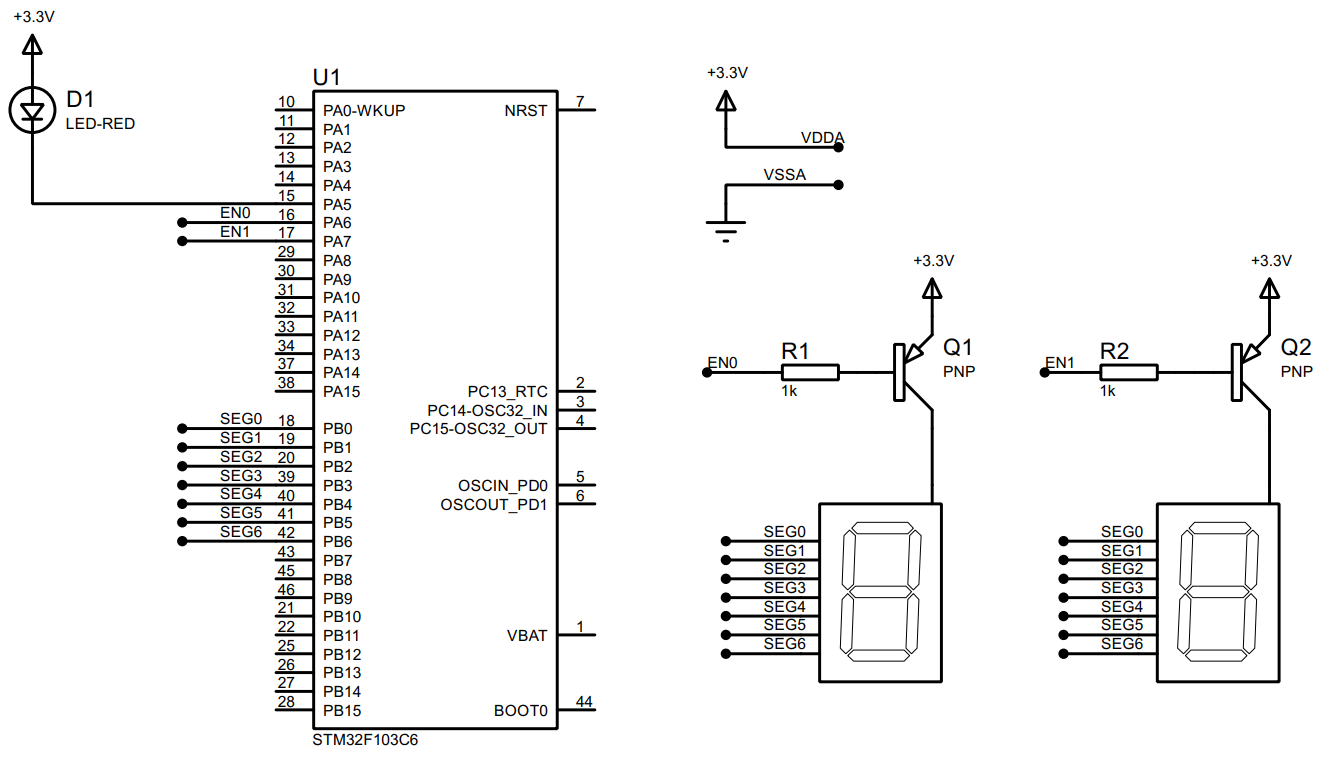
\includegraphics[width=5.5in]{source/picture/bai_2/lab2_ex1a.PNG}
    \caption{\textit{Simulation schematic in Proteus}}
    \label{bai2_pic1a}
\end{figure}
Components used in the schematic are listed bellow:
\begin{itemize}
    \item 7SEG-COM-ANODE (connected from PB0 to PB6)
    \item LED-RED
    \item PNP
    \item RES
    \item STM32F103C6
\end{itemize}


Students are proposed to use the function \textbf{display7SEG(int num)} in the Lab 1 in this exercise. Implement the source code in the interrupt callback function to display number \textbf{"1"} on the first seven segment and number \textbf{"2"} for second one. The switching time between 2 LEDs is half of second. \\

\textbf{Report 1: } The Proteus circuit uses two common-anode seven-segment displays. Their seven cathode signals are shared and connected to \textbf{PB0--PB6}, labelled \textbf{SEG0--SEG6}. The common anode of each display is supplied from 3.3V through a PNP high-side switch. The bases of the two PNP transistors are controlled by \textbf{PA6 (EN0)} and \textbf{PA7 (EN1)}. Because the PNP enable signals are active-low, writing logic 0 to an enable pin selects that display, while logic 1 switches it off.

Only one display is enabled at a time. Before changing the segment pattern, the program disables both displays to prevent ghosting, writes the new active-low segment data, and then enables the selected display. Figures~\ref{bai2_ex1_display_1} and~\ref{bai2_ex1_display_2} show the two states captured during the simulation.

\begin{figure}[!htp]
    \centering
    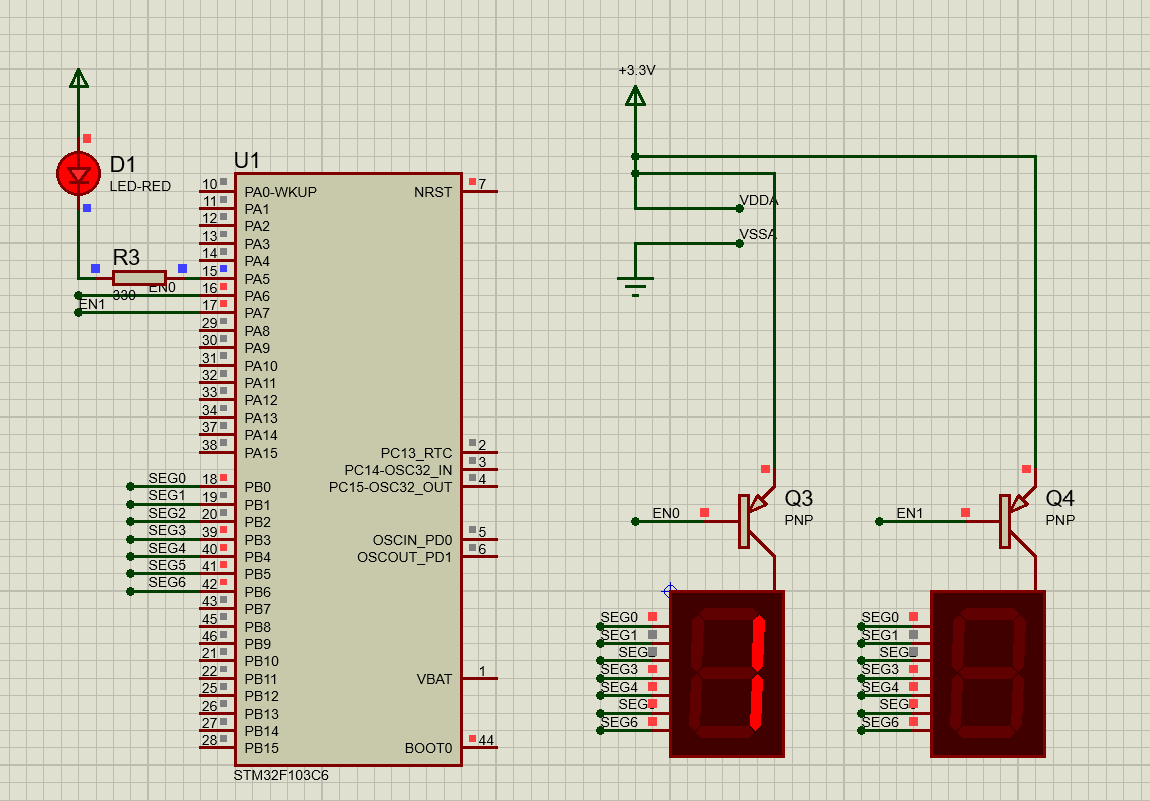
\includegraphics[width=5.5in]{source/picture/bai_2/lab2_ex1.1.png}
    \caption{\href{https://raw.githubusercontent.com/quangnguyencomeng/CO3009-261-CC-2453052/main/Lab/LAB02/PROTEUS/lab2.pdsprj}{\textit{Proteus simulation displaying number 1 on the first seven-segment display (download project)}}}
    \label{bai2_ex1_display_1}
\end{figure}

\begin{figure}[!htp]
    \centering
    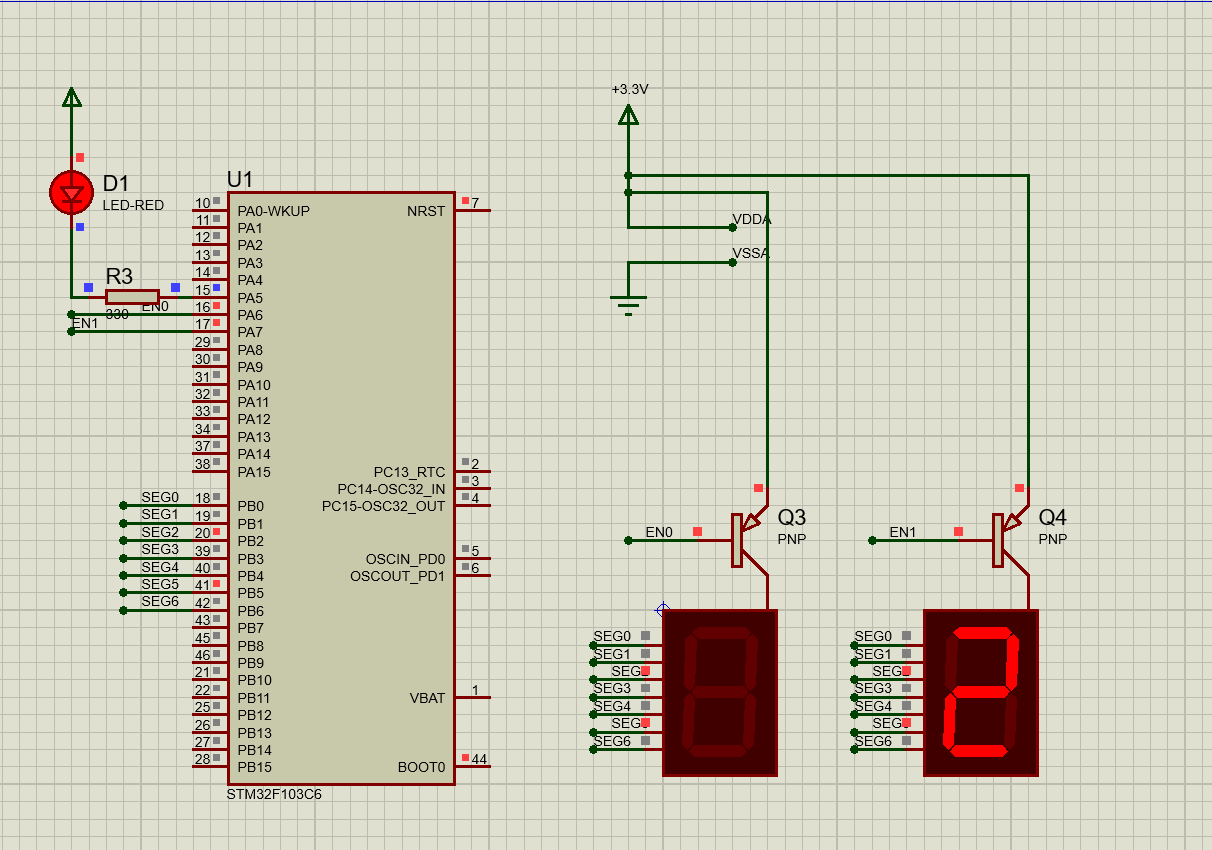
\includegraphics[width=5.5in]{source/picture/bai_2/lab2_ex1.2.png}
    \caption{\textit{Proteus simulation displaying number 2 on the second seven-segment display}}
    \label{bai2_ex1_display_2}
\end{figure}

The demonstration video for this exercise is available at:
\begin{center}
    \url{https://github.com/quangnguyencomeng/CO3009-261-CC-2453052/blob/main/Lab/lab_reports/source/vids/lab2_ex1.mp4}
\end{center}

\textbf{Report 2: } The exercise specifically requires the implementation of \texttt{HAL\_TIM\_PeriodElapsedCallback()}. The callback uses the two state variables below. The \texttt{timer2\_ticks} variable counts 10 ms timer interrupts, while \texttt{active\_display} records which seven-segment display is currently selected. They are declared \texttt{volatile} because they are updated from interrupt-driven code.

\begin{lstlisting}[caption={State variables used by the Timer 2 callback}]
volatile uint8_t active_display = 0U;
volatile uint8_t timer2_ticks = 0U;
\end{lstlisting}

The \texttt{display7SEG()} function is reused from Lab 1 to generate the active-low segment pattern and is therefore not repeated in this report. The following directly related helper performs the display selection. It first drives both PNP enable pins HIGH to disable both displays, changes the shared segment data, and finally drives the selected enable pin LOW. Disabling both displays before changing the segment pattern prevents ghosting.

\begin{lstlisting}[caption={Selecting one display through the active-low PNP enables}]
void show7SEG(uint8_t display, int num)
{
  /* Disable both displays before changing the segment data. */
  HAL_GPIO_WritePin(GPIOA, EN0_Pin | EN1_Pin, GPIO_PIN_SET);
  display7SEG(num);

  if (display == 0U)
  {
    HAL_GPIO_WritePin(EN0_GPIO_Port, EN0_Pin, GPIO_PIN_RESET);
  }
  else
  {
    HAL_GPIO_WritePin(EN1_GPIO_Port, EN1_Pin, GPIO_PIN_RESET);
  }
}
\end{lstlisting}

Timer 2 generates an interrupt every 10 ms. The required callback counts 50 interrupts to obtain the 500 ms switching interval. It then alternates between the first display showing number 1 and the second display showing number 2.

\begin{lstlisting}[caption={Timer callback for scanning the two seven-segment displays}]
void HAL_TIM_PeriodElapsedCallback(TIM_HandleTypeDef *htim)
{
  if (htim->Instance != TIM2)
  {
    return;
  }

  timer2_ticks++;
  if (timer2_ticks >= 50U)  /* 50 x 10 ms = 500 ms */
  {
    timer2_ticks = 0U;

    if (active_display == 0U)
    {
      show7SEG(1U, 2);
      active_display = 1U;
    }
    else
    {
      show7SEG(0U, 1);
      active_display = 0U;
    }
  }
}
\end{lstlisting}

The initial display is selected and the timer interrupt is started after the GPIO and Timer 2 peripherals have been initialized:

\begin{lstlisting}[caption={Starting the first display and Timer 2 interrupt}]
show7SEG(0U, 1);
HAL_TIM_Base_Start_IT(&htim2);
\end{lstlisting}

\textbf{Short question: What is the frequency of the scanning process?}

The Timer 2 interrupt frequency is
\[
f_{\mathrm{TIM2}}
= \frac{8\,\mathrm{MHz}}{(7999+1)(9+1)}
= 100\,\mathrm{Hz},
\]
so one interrupt occurs every 10 ms. A display remains selected for
\[
T_S = 50 \times 10\,\mathrm{ms} = 0.5\,\mathrm{s}.
\]
For two displays, one complete scan takes
\[
T_{\mathrm{scan}} = 2T_S = 1\,\mathrm{s}.
\]
Therefore, the scanning frequency is
\[
\boxed{f_{\mathrm{scan}} = \frac{1}{T_{\mathrm{scan}}} = 1\,\mathrm{Hz}}.
\]
The display-selection event occurs every 0.5 s (2 Hz), but a full cycle that visits both displays repeats once per second.

\subsubsection{Exercise 2}
Extend to 4 seven segment LEDs and two LEDs (connected to PA4, labeled as \textbf{DOT}) in the middle as following:

\begin{figure}[!htp]
    \centering
    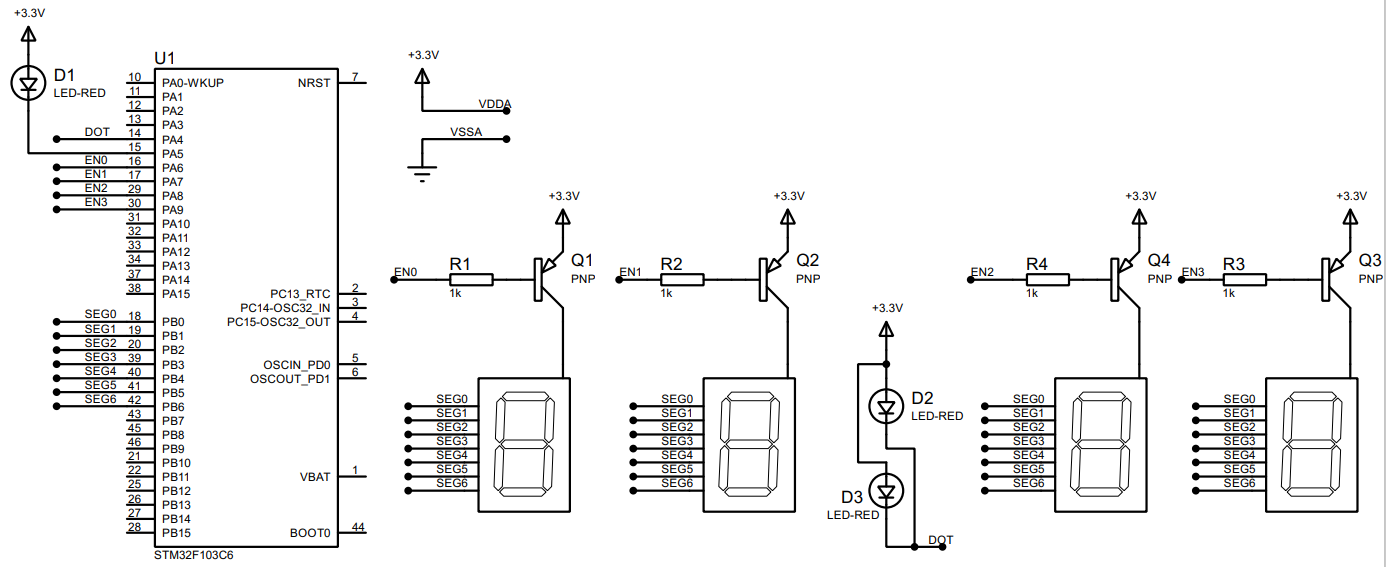
\includegraphics[width=5.5in]{source/picture/bai_2/lab2_ex2a.PNG}
    \caption{\textit{Simulation schematic in Proteus}}
    \label{bai2_pic2a}
\end{figure}

Blink the two LEDs every second. Meanwhile, number 3 is displayed on the third seven segment and number 0 is displayed on the last one (to present 12 hour and a half). The switching time for each seven segment LED is also a half of second (500ms). \textbf{Implement your code in the timer interrupt function.}\\

\textbf{Report 1: } The circuit is extended with two additional common-anode seven-segment displays. Their segment inputs remain connected to the shared \textbf{SEG0--SEG6} bus on \textbf{PB0--PB6}. The four active-low PNP enable signals are mapped to \textbf{PA6 (EN0)}, \textbf{PA7 (EN1)}, \textbf{PA8 (EN2)}, and \textbf{PA9 (EN3)}. The two red LEDs in the middle share the active-low \textbf{DOT} control on \textbf{PA4}, so driving PA4 LOW turns the dots on and driving it HIGH turns them off.

The DOT signal is separate from the four seven-segment values: the first two displays show ``12'', the two LEDs controlled by PA4 form the colon in the middle, and the last two displays show ``30''. The pin assignment generated from the STM32 configuration is:

\begin{lstlisting}[caption={GPIO assignment for the two center DOT LEDs}]
#define DOT_Pin        GPIO_PIN_4
#define DOT_GPIO_Port  GPIOA
\end{lstlisting}

PA4 is configured as a push-pull GPIO output. Since the two DOT LEDs are active-low, the initial HIGH level keeps them off. The callback drives PA4 LOW only during the dedicated DOT slot between the second and third digits:

\begin{lstlisting}[caption={Initialization of the active-low DOT output}]
/* The two center LEDs share the active-low DOT signal on PA4. */
HAL_GPIO_WritePin(DOT_GPIO_Port, DOT_Pin, GPIO_PIN_SET);

GPIO_InitStruct.Pin = DOT_Pin | LED_RED_Pin | EN0_Pin | EN1_Pin
                    | EN2_Pin | EN3_Pin;
GPIO_InitStruct.Mode = GPIO_MODE_OUTPUT_PP;
GPIO_InitStruct.Pull = GPIO_NOPULL;
GPIO_InitStruct.Speed = GPIO_SPEED_FREQ_LOW;
HAL_GPIO_Init(GPIOA, &GPIO_InitStruct);
\end{lstlisting}

The four display values are 1, 2, 3, and 0, producing the clock-like result ``12:30''. Only one display or the DOT pair is enabled at a time. Figure~\ref{bai2_ex2_schematic} shows the completed Proteus implementation with the shared segment bus, four PNP high-side switches, and the two center LEDs connected to the DOT net.

\begin{figure}[!htp]
    \centering
    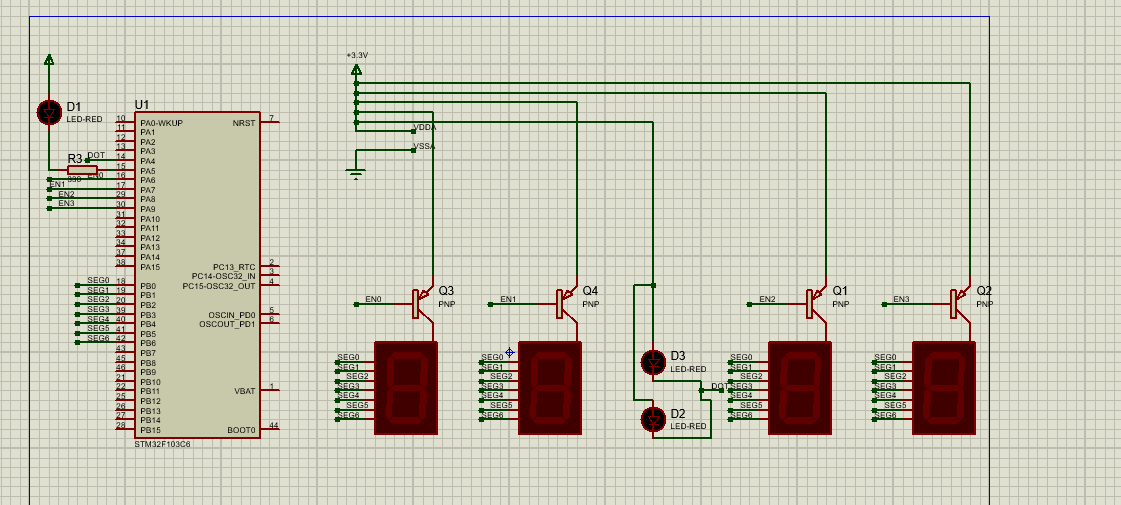
\includegraphics[width=5.5in]{source/picture/bai_2/lab2_ex2.png}
    \caption{\href{https://raw.githubusercontent.com/quangnguyencomeng/CO3009-261-CC-2453052/main/Lab/LAB02/PROTEUS/lab2.pdsprj}{\textit{Completed Proteus schematic for Exercise 2 (download project)}}}
    \label{bai2_ex2_schematic}
\end{figure}

The simulation recording demonstrates the complete sequence \textbf{1, 2, DOT, 3, 0}. It is available at:
\begin{center}
    \url{https://github.com/quangnguyencomeng/CO3009-261-CC-2453052/blob/main/Lab/lab_reports/source/vids/lab2_ex2.mp4}
\end{center}

\textbf{Report 2: } Exercise 2 requires the updated \texttt{HAL\_TIM\_PeriodElapsedCallback()}. The implementation uses a five-step state machine so that the visible sequence is exactly \textbf{1, 2, DOT, 3, 0}. The timer counter creates a 500 ms interval for every state.

\begin{lstlisting}[caption={State used by the five-step scanning sequence}]
volatile uint8_t scan_step = 0U;
volatile uint8_t timer2_ticks = 0U;
\end{lstlisting}

The \texttt{show7SEG()} helper from Exercise 1 is extended to disable \texttt{EN0--EN3} before updating the shared segment bus and then enable only the selected PNP switch. In the DOT state, all four PNP switches and all seven segments are disabled, and PA4 alone is driven LOW. The callback itself is shown below, as requested by the exercise.

\begin{lstlisting}[caption={Timer callback for Exercise 2}]
void HAL_TIM_PeriodElapsedCallback(TIM_HandleTypeDef *htim)
{
  if (htim->Instance != TIM2)
  {
    return;
  }

  timer2_ticks++;

  if (timer2_ticks >= 50U)  /* 50 x 10 ms = 500 ms */
  {
    timer2_ticks = 0U;
    scan_step = (scan_step + 1U) % 5U;

    /* DOT is active only in its own slot between digits 2 and 3. */
    HAL_GPIO_WritePin(DOT_GPIO_Port, DOT_Pin, GPIO_PIN_SET);

    switch (scan_step)
    {
      case 0U:
        show7SEG(0U, 1);
        break;
      case 1U:
        show7SEG(1U, 2);
        break;
      case 2U:
        HAL_GPIO_WritePin(GPIOA,
                          EN0_Pin | EN1_Pin | EN2_Pin | EN3_Pin,
                          GPIO_PIN_SET);
        display7SEG(-1);
        HAL_GPIO_WritePin(DOT_GPIO_Port, DOT_Pin, GPIO_PIN_RESET);
        break;
      case 3U:
        show7SEG(2U, 3);
        break;
      case 4U:
        show7SEG(3U, 0);
        break;
      default:
        break;
    }
  }
}
\end{lstlisting}

At startup, the first display shows number 1. Every 500 ms the state advances to number 2, the two DOT LEDs, number 3, and number 0 before returning to number 1.

\textbf{Short question: What is the frequency of the scanning process?}

Every state is selected for $T_S=0.5\,\mathrm{s}$. Because the requested sequence contains four display states and one separate DOT state, one complete sequence takes
\[
T_{\mathrm{sequence}} = 5T_S = 5 \times 0.5\,\mathrm{s} = 2.5\,\mathrm{s}.
\]
Thus, the repetition frequency of the implemented sequence is
\[
\boxed{f_{\mathrm{sequence}} = \frac{1}{T_{\mathrm{sequence}}} = 0.4\,\mathrm{Hz}}.
\]
The state-selection rate remains 2 Hz. If only the four seven-segment displays were counted and the DOT state were excluded, their nominal scan frequency would be $1/(4T_S)=0.5\,\mathrm{Hz}$; however, the actual five-state sequence requested here repeats at 0.4 Hz.

\subsubsection{Exercise 3}
Implement a function named \textbf{update7SEG(int index)}. An array of 4 integer numbers are declared in this case. The code skeleton in this exercise is presented as following:

Exercise 3 separates the display data from the multiplexing logic. The \texttt{led\_buffer} array stores the value assigned to each physical display, while \texttt{index\_led} identifies the display that is refreshed during the current scanning interval. Changing the array values is therefore sufficient to test a different four-digit pattern; the scanning code does not need to be rewritten.

\begin{lstlisting}[caption={Display buffer and scanning index for Exercise 3}]
const int MAX_LED = 4;
volatile int index_led = 0;
int led_buffer[4] = {1, 2, 3, 4};
volatile uint8_t scan_step = 0U;
\end{lstlisting}

\textbf{Report 1: } The \texttt{update7SEG()} function selects one of the four physical displays and sends the corresponding buffered value to \texttt{show7SEG()}. The helper inherited from the previous exercises disables all PNP switches before updating the shared segment bus, so changing from one display to the next does not cause ghosting.

\begin{lstlisting}[caption={Implementation of update7SEG for Exercise 3}]
void update7SEG(int index)
{
  switch (index)
  {
    case 0:
      show7SEG(0U, led_buffer[0]);
      break;
    case 1:
      show7SEG(1U, led_buffer[1]);
      break;
    case 2:
      show7SEG(2U, led_buffer[2]);
      break;
    case 3:
      show7SEG(3U, led_buffer[3]);
      break;
    default:
      break;
  }
}
\end{lstlisting}

\textbf{Report 2: } Timer 2 still raises an interrupt every 10 ms. Fifty interrupts produce the 500 ms interval used for the visible Proteus test. Because Exercise 3 does not request any change to the DOT behavior, the five-step sequence from Exercise 2 is preserved. The digit states now call \texttt{update7SEG()} with indices 0, 1, 2, and 3, while the middle state disables all four displays and enables only the DOT pair. The resulting sequence is \textbf{1, 2, DOT, 3, 4}.

\begin{lstlisting}[caption={Timer callback using update7SEG in Exercise 3}]
void HAL_TIM_PeriodElapsedCallback(TIM_HandleTypeDef *htim)
{
  if (htim->Instance != TIM2)
  {
    return;
  }

  timer2_ticks++;

  if (timer2_ticks >= 50U)  /* 50 x 10 ms = 500 ms */
  {
    timer2_ticks = 0U;
    scan_step = (scan_step + 1U) % 5U;

    /* Preserve the Exercise 2 sequence: 1, 2, DOT, 3, 4. */
    HAL_GPIO_WritePin(DOT_GPIO_Port, DOT_Pin, GPIO_PIN_SET);

    switch (scan_step)
    {
      case 0U:
        index_led = 0;
        update7SEG(index_led);
        break;
      case 1U:
        index_led = 1;
        update7SEG(index_led);
        break;
      case 2U:
        HAL_GPIO_WritePin(GPIOA,
                          EN0_Pin | EN1_Pin | EN2_Pin | EN3_Pin,
                          GPIO_PIN_SET);
        display7SEG(-1);
        HAL_GPIO_WritePin(DOT_GPIO_Port, DOT_Pin, GPIO_PIN_RESET);
        break;
      case 3U:
        index_led = 2;
        update7SEG(index_led);
        break;
      case 4U:
        index_led = 3;
        update7SEG(index_led);
        break;
      default:
        break;
    }
  }
}
\end{lstlisting}

The first test uses \texttt{led\_buffer = \{1, 2, 3, 4\}}. During multiplexing, the four stored digits are displayed in order, while the DOT state is inserted between the second and third digits. Therefore, the complete visible sequence is \textbf{1--2--DOT--3--4}, as shown in Figure~\ref{fig:ex3-initial-sequence}.

\begin{figure}[!htp]
    \centering
    \begin{minipage}[t]{0.19\textwidth}
        \centering
        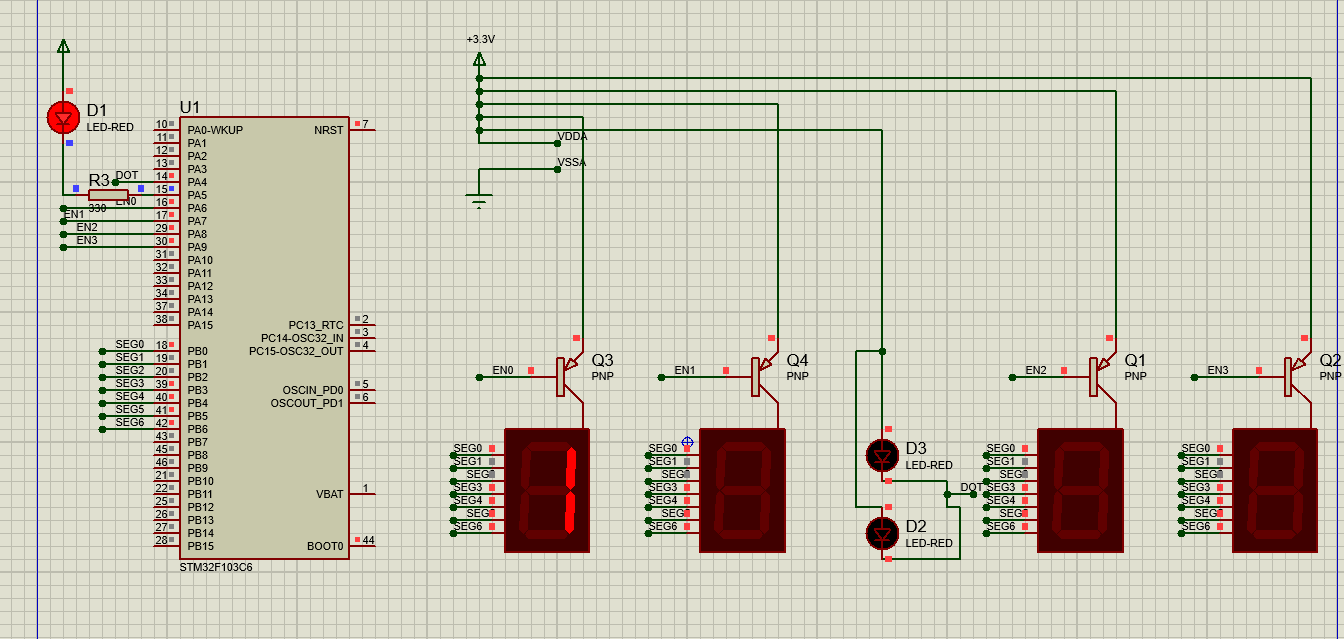
\includegraphics[width=\linewidth]{source/picture/bai_2/lab2_ex3_1.png}\\[-1mm]
        \scriptsize (a) Digit 1
    \end{minipage}\hfill
    \begin{minipage}[t]{0.19\textwidth}
        \centering
        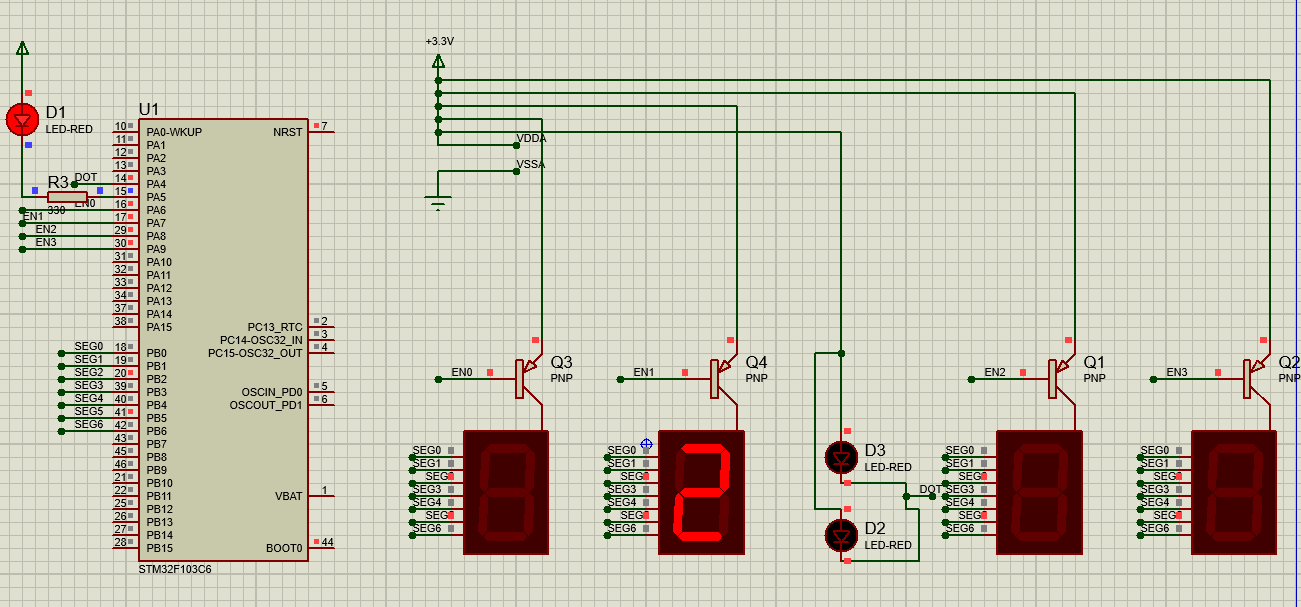
\includegraphics[width=\linewidth]{source/picture/bai_2/lab2_ex3_2.png}\\[-1mm]
        \scriptsize (b) Digit 2
    \end{minipage}\hfill
    \begin{minipage}[t]{0.19\textwidth}
        \centering
        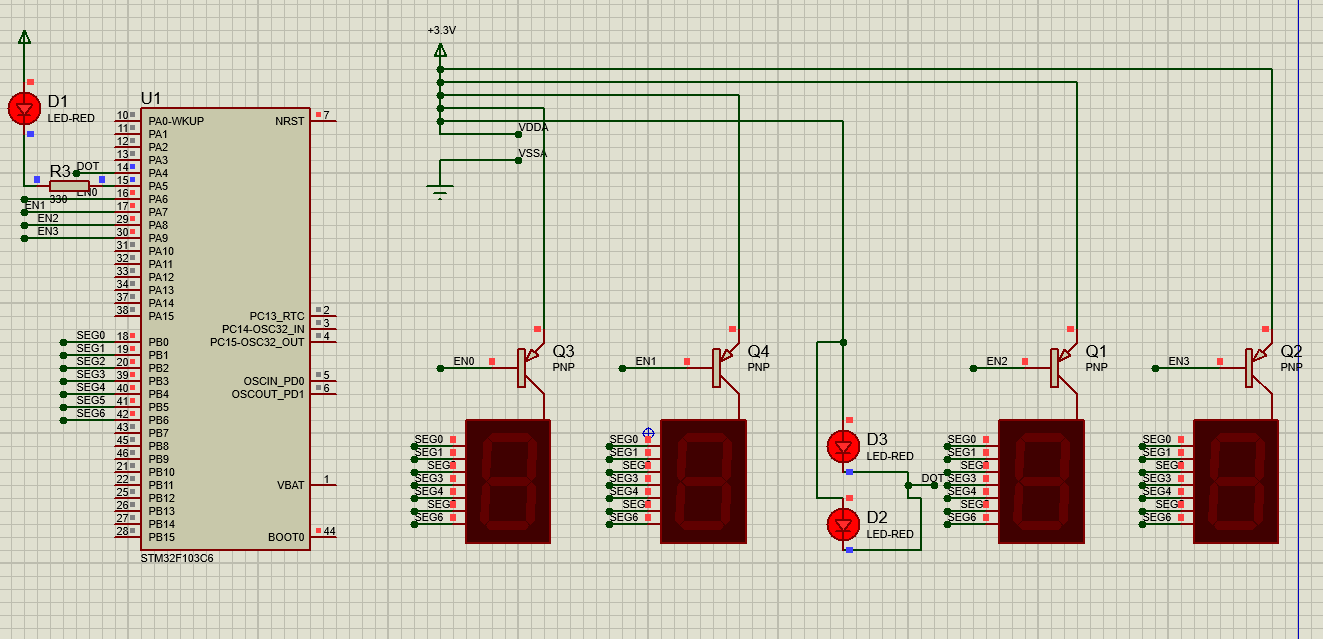
\includegraphics[width=\linewidth]{source/picture/bai_2/lab2_ex3_dot.png}\\[-1mm]
        \scriptsize (c) DOT
    \end{minipage}\hfill
    \begin{minipage}[t]{0.19\textwidth}
        \centering
        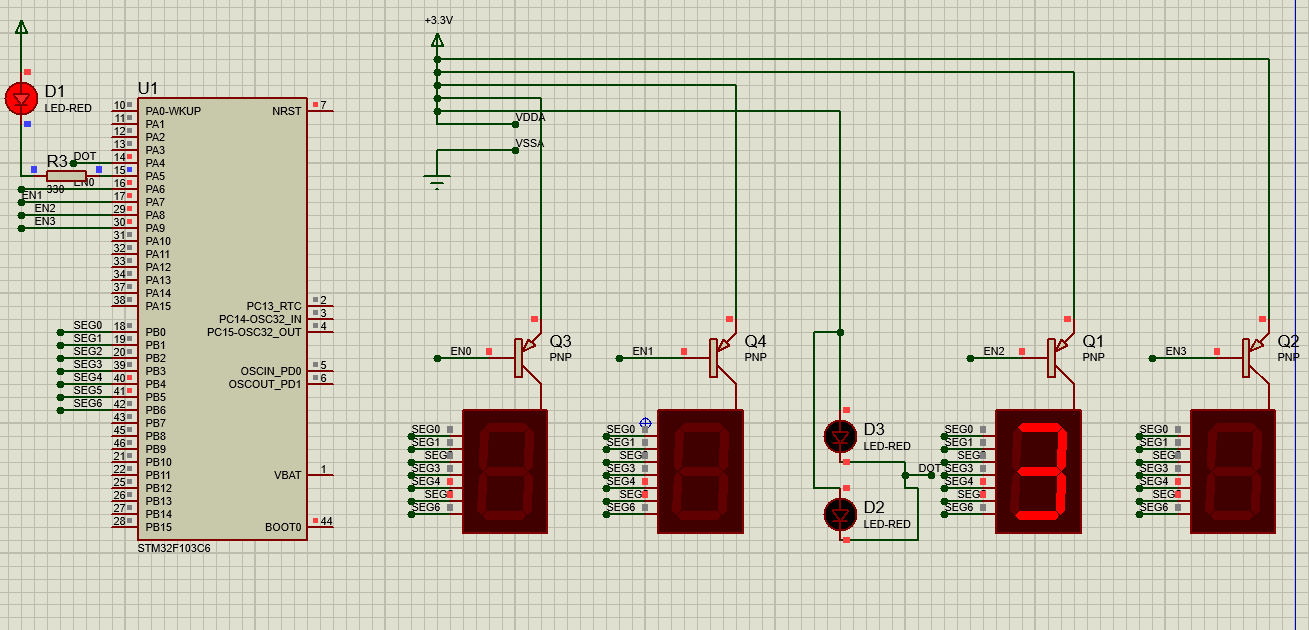
\includegraphics[width=\linewidth]{source/picture/bai_2/lab2_ex3_3.png}\\[-1mm]
        \scriptsize (d) Digit 3
    \end{minipage}\hfill
    \begin{minipage}[t]{0.19\textwidth}
        \centering
        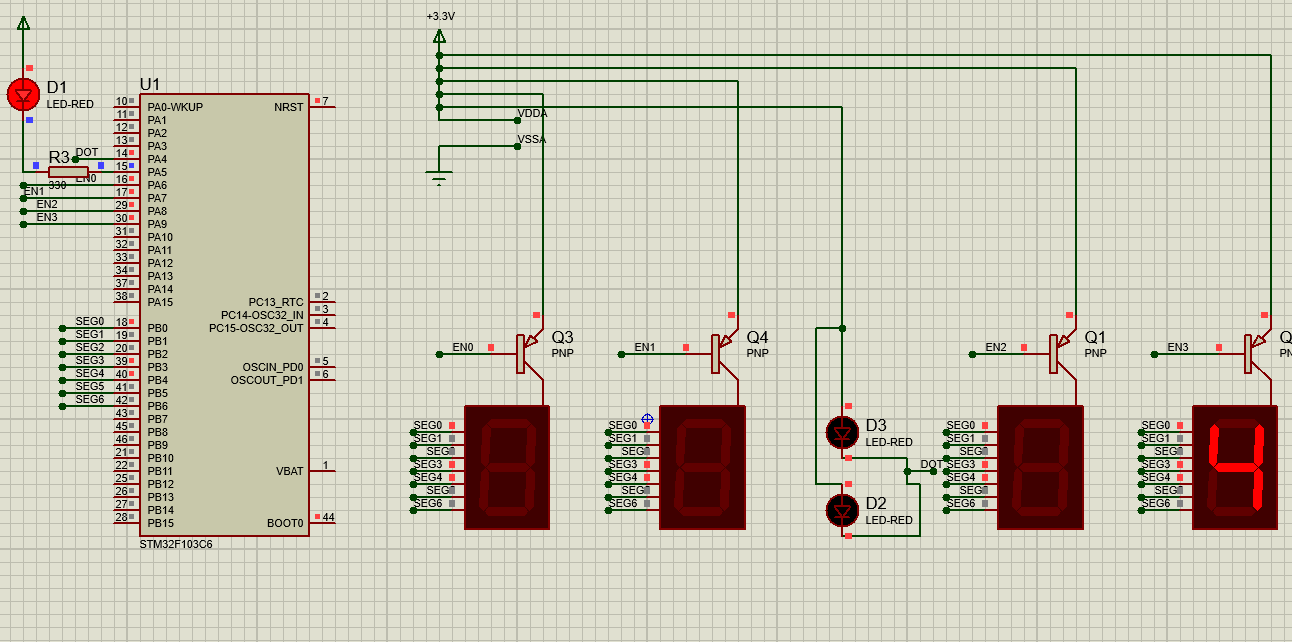
\includegraphics[width=\linewidth]{source/picture/bai_2/lab2_ex3_4.png}\\[-1mm]
        \scriptsize (e) Digit 4
    \end{minipage}
    \caption{\textit{Five successive display states for the initial buffer: 1--2--DOT--3--4.}}
    \label{fig:ex3-initial-sequence}
\end{figure}

To verify that the displayed values are obtained from the buffer rather than fixed directly in the scanning routine, the buffer is changed to \texttt{\{3, 6, 6, 9\}}, as shown in Figure~\ref{fig:ex3-buffer-update}. No change is required in \texttt{update7SEG()} or in the timer callback.

\begin{figure}[!htp]
    \centering
    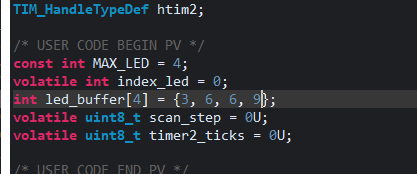
\includegraphics[width=0.62\textwidth]{source/picture/bai_2/lab2_ex3_update.png}
    \caption{\textit{Updating the four display values in \texttt{led\_buffer} to 3, 6, 6, and 9.}}
    \label{fig:ex3-buffer-update}
\end{figure}

After rebuilding and running the simulation, the multiplexing order becomes \textbf{3--6--DOT--6--9}, as presented in Figure~\ref{fig:ex3-updated-sequence}. The same DOT state is retained between the second and third buffered digits. The suffix \texttt{\_1} in some image filenames is used only to avoid duplicate filenames; it does not denote an additional display state.

\begin{figure}[!htp]
    \centering
    \begin{minipage}[t]{0.19\textwidth}
        \centering
        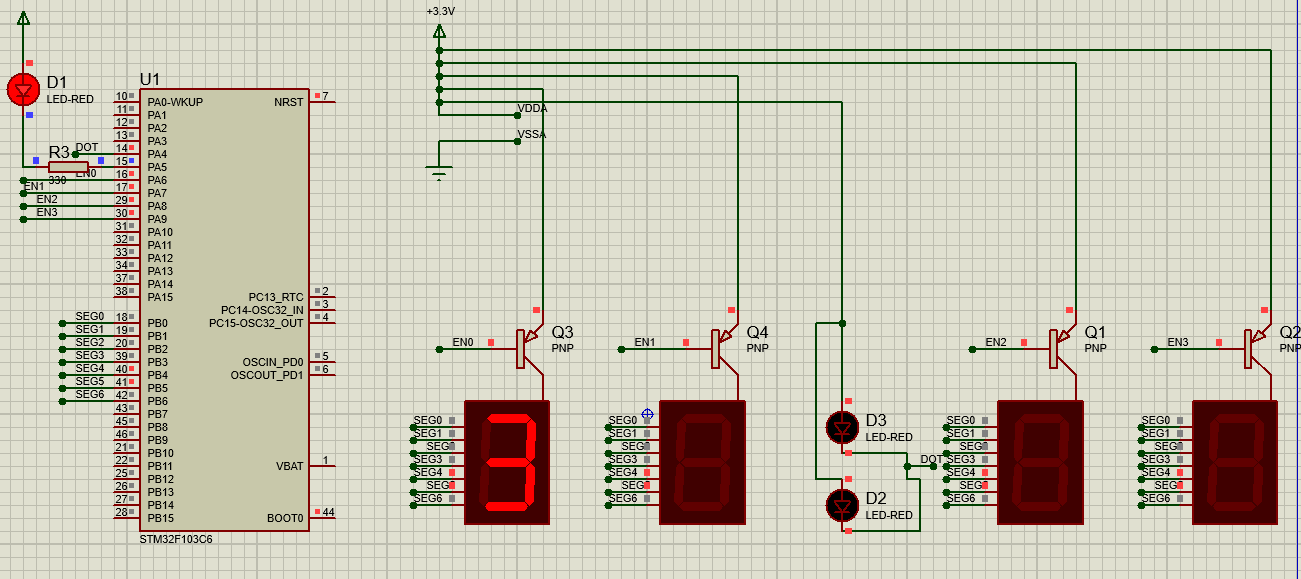
\includegraphics[width=\linewidth]{source/picture/bai_2/lab2_ex3_3_1.png}\\[-1mm]
        \scriptsize (a) Digit 3
    \end{minipage}\hfill
    \begin{minipage}[t]{0.19\textwidth}
        \centering
        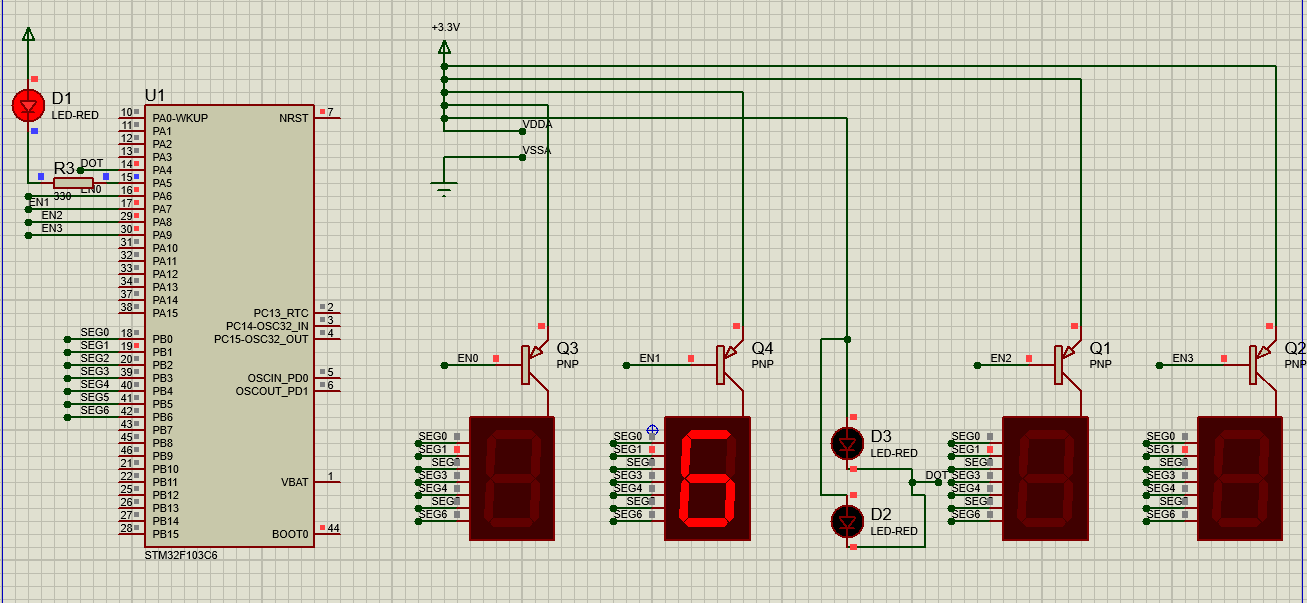
\includegraphics[width=\linewidth]{source/picture/bai_2/lab2_ex3_6.png}\\[-1mm]
        \scriptsize (b) First digit 6
    \end{minipage}\hfill
    \begin{minipage}[t]{0.19\textwidth}
        \centering
        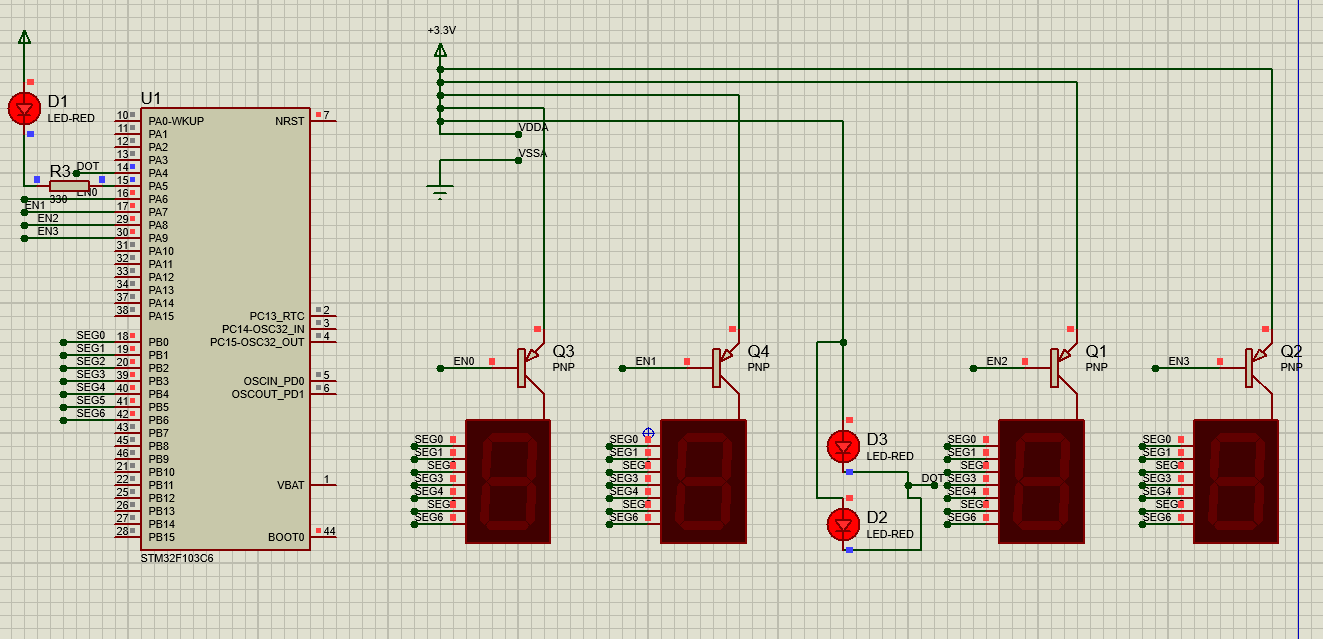
\includegraphics[width=\linewidth]{source/picture/bai_2/lab2_ex3_dot.png}\\[-1mm]
        \scriptsize (c) DOT
    \end{minipage}\hfill
    \begin{minipage}[t]{0.19\textwidth}
        \centering
        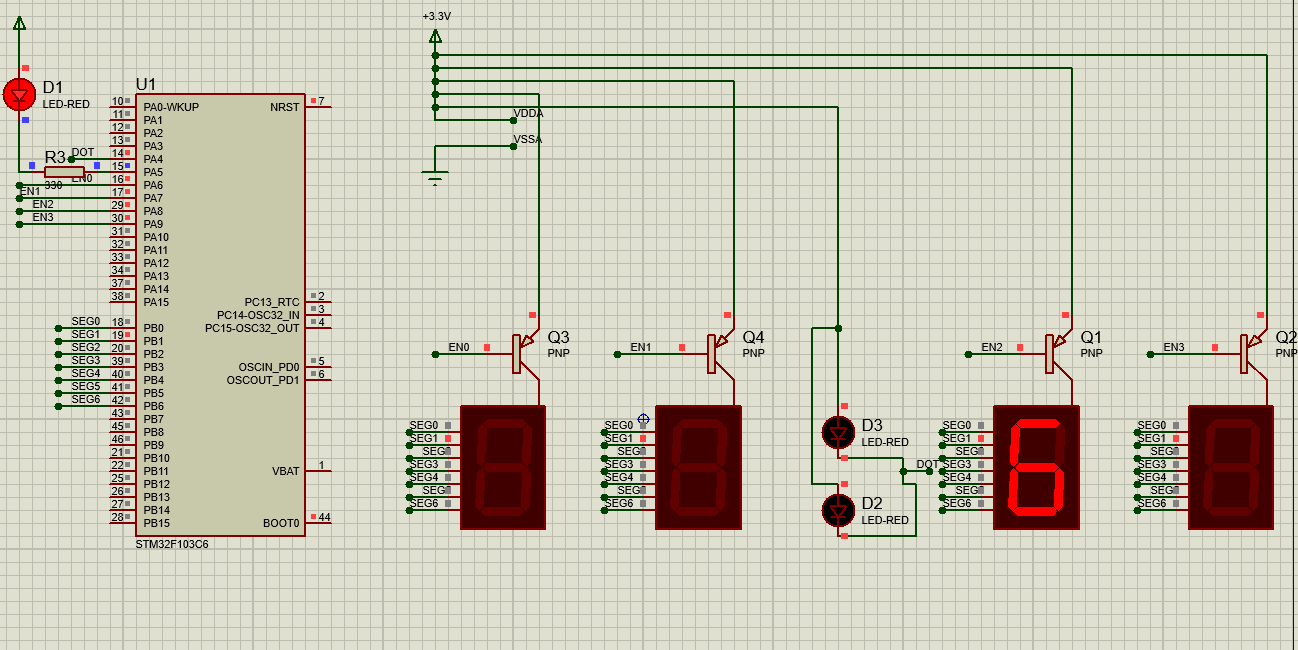
\includegraphics[width=\linewidth]{source/picture/bai_2/lab2_ex3_6_1.png}\\[-1mm]
        \scriptsize (d) Second digit 6
    \end{minipage}\hfill
    \begin{minipage}[t]{0.19\textwidth}
        \centering
        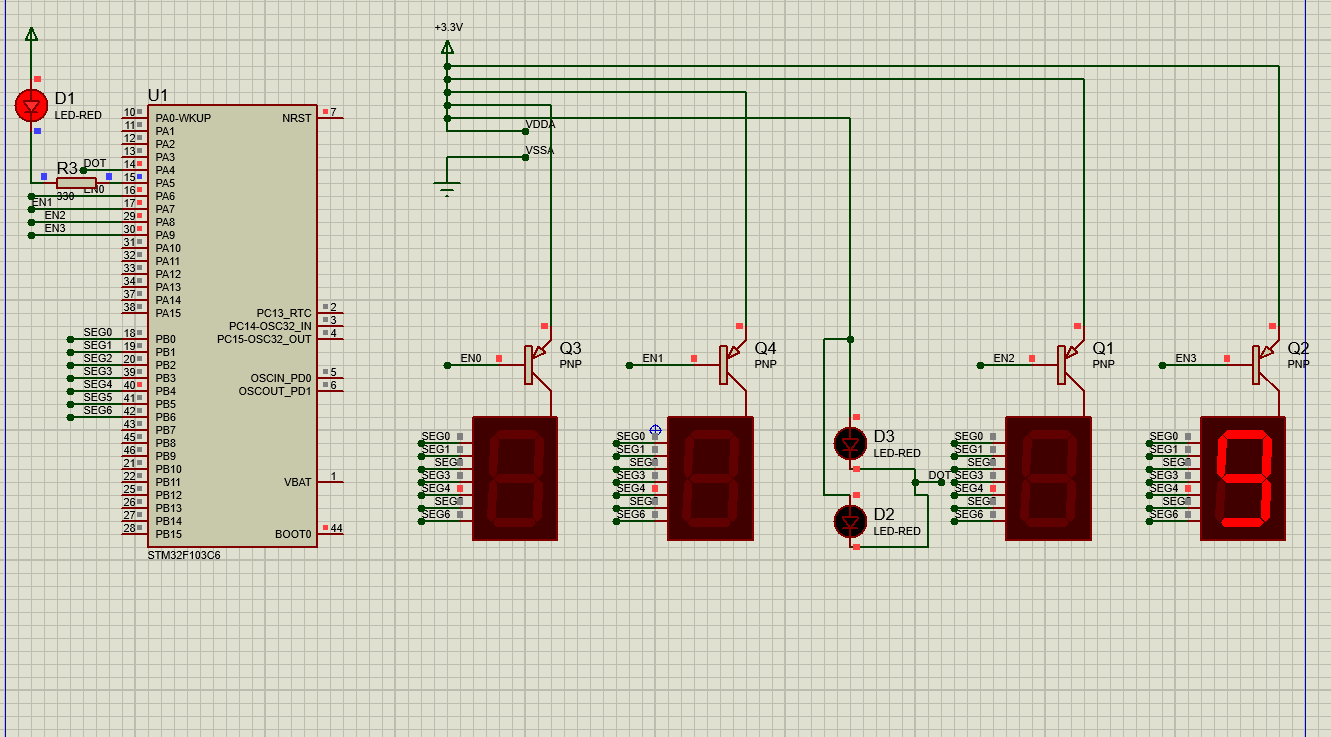
\includegraphics[width=\linewidth]{source/picture/bai_2/lab2_ex3_9.png}\\[-1mm]
        \scriptsize (e) Digit 9
    \end{minipage}
    \caption{\textit{Five successive display states after updating the buffer: 3--6--DOT--6--9.}}
    \label{fig:ex3-updated-sequence}
\end{figure}

The complete operation of Exercise 3 is recorded in the following video:
\begin{center}
    \href{https://github.com/quangnguyencomeng/CO3009-261-CC-2453052/blob/main/Lab/lab_reports/source/vids/lab2_ex3.mp4}{\textbf{Exercise 3 demonstration video}}
\end{center}

% Exercise 3 is the completed scope of the current Lab 2 report.
\subsubsection{Exercise 4}

Change the period of invoking update7SEG function in order to set the frequency of 4 seven segment LEDs to 1Hz. The DOT is still blinking every second.\\

\textbf{Report 1: } Present the source code in the \textbf{HAL\_TIM\_PeriodElapsedCallback}. \\

Exercise 4 requires the DOT to blink every second while the four seven-segment displays remain visually continuous. Therefore, the display multiplexing must be much faster than the one-second time base: with a TIM2 interrupt period of \SI{10}{ms}, the next display is selected on every interrupt. The four positions are consequently refreshed at a complete-frame rate of \SI{25}{Hz}, which avoids visible flicker. The DOT uses a separate counter of 100 interrupts and is toggled once every \SI{1}{s}; it is not inserted as a fifth scanning state.

\paragraph{Report 1: Source code in \texttt{HAL\_TIM\_PeriodElapsedCallback()}.}

\begin{lstlisting}[caption={Fast four-display multiplexing and a DOT toggled every second}]
void HAL_TIM_PeriodElapsedCallback(TIM_HandleTypeDef *htim)
{
  static uint8_t scan_tick_count = 0U;
  static uint8_t dot_tick_count = 0U;

  if (htim->Instance != TIM2)
  {
    return;
  }

  // Select the next display on every 10 ms interrupt.
  scan_tick_count++;
  if (scan_tick_count >= 1U)
  {
    scan_tick_count = 0U;
    update7SEG(index_led);
    index_led = (index_led + 1) % MAX_LED;
  }

  // 100 x 10 ms = 1 s between DOT state changes
  dot_tick_count++;
  if (dot_tick_count >= 100U)
  {
    dot_tick_count = 0U;
    HAL_GPIO_TogglePin(GPIOA, DOT_Pin);
  }
}
\end{lstlisting}

The two counters operate independently: changing the active seven-segment display does not affect the DOT timing, and toggling the DOT does not add an extra state to the four-display scan. The four displays therefore appear continuously, while the DOT alternates between ON and OFF every second. When the minute or hour changes, \texttt{updateClockBuffer()} writes the new digits to \texttt{led\_buffer}; the next multiplexing cycles immediately show the updated value.

Compared with Exercise 3, the DOT is no longer treated as one of the display positions. The scan sequence contains only indices 0--3, so all four digit positions are refreshed continuously. The DOT state is controlled by its own one-second counter, which prevents DOT blinking from disturbing the digit refresh. This separation is also the reason that a change in the clock buffer can be displayed immediately without changing the scanning routine.

\subsubsection{Exercise 5}

Exercise 5 extends the multiplexed display into a digital clock. The four positions show time in the \textbf{HH:MM} format: the first two entries of \texttt{led\_buffer} contain the hour, and the last two entries contain the minute. The clock is initialized to \texttt{15:08:50}. Every second, \texttt{second} is incremented and the following rollover rules are applied:
\begin{itemize}
    \item at 60 seconds, \texttt{second} returns to 0 and \texttt{minute} increases by one;
    \item at 60 minutes, \texttt{minute} returns to 0 and \texttt{hour} increases by one;
    \item at 24 hours, \texttt{hour} returns to 0.
\end{itemize}
After updating the time, \texttt{updateClockBuffer()} converts the current hour and minute into four decimal digits. Integer division produces the tens digit, whereas the remainder operator produces the units digit. Therefore, one-digit values are automatically displayed with a leading zero; for example, \texttt{7:05} produces the buffer \texttt{\{0, 7, 0, 5\}}.

\paragraph{Report 1: Source code of \texttt{updateClockBuffer()}.}

\begin{lstlisting}[caption={Conversion from hour and minute values to the four-digit display buffer}]
/* Minute rollover test: 15:08:50 */
int hour = 15;
int minute = 8;
int second = 50;

void updateClockBuffer(void)
{
  led_buffer[0] = hour / 10;
  led_buffer[1] = hour % 10;
  led_buffer[2] = minute / 10;
  led_buffer[3] = minute % 10;
}
\end{lstlisting}

The main loop follows the code skeleton provided in the exercise: it increments the time, performs the rollover checks, calls \texttt{updateClockBuffer()}, and then waits for \SI{1}{s} using \texttt{HAL\_Delay(1000)}. The TIM2 interrupt continues multiplexing the four displays and toggling the DOT every second. Consequently, timekeeping and buffer generation are separated from the low-level display-selection operation. The blocking delay is retained in this exercise as requested; it will be replaced by a software timer in the subsequent exercises.

Two initial values were used to verify both rollover cases. For the minute transition, the program was initialized as \texttt{15:08:50}; after ten seconds it reaches \texttt{15:09:00}. For the hour transition, only the initial minute value was changed to obtain \texttt{15:59:50}; after ten seconds the display rolls over to \texttt{16:00:00}. The corresponding Proteus demonstrations are linked below.

\begin{center}
    \href{https://github.com/quangnguyencomeng/CO3009-261-CC-2453052/blob/main/Lab/lab_reports/source/vids/lab2_ex5_min.mp4}{\textbf{Exercise 5 -- minute rollover video}}\\[2mm]
    \href{https://github.com/quangnguyencomeng/CO3009-261-CC-2453052/blob/main/Lab/lab_reports/source/vids/lab2_ex5_hour.mp4}{\textbf{Exercise 5 -- hour rollover video}}
\end{center}



\subsubsection{Exercise 6}

Exercise 6 introduces a \textbf{software timer} built on the existing TIM2 hardware timer. TIM2 still generates an interrupt every \SI{10}{ms}, but instead of using \texttt{HAL\_Delay()} to block the main program, the interrupt only decreases a software counter. When the counter reaches zero, a flag is raised. The main loop continuously checks this flag and performs the required task when the timer expires. Therefore, the timing source is interrupt-driven, while the flag is checked by polling in \texttt{while(1)}.

The purpose of this exercise is to create a non-blocking timing mechanism that can later replace \texttt{HAL\_Delay(1000)} in the digital clock. The hour/minute update from Exercise 5 is intentionally not moved to the software timer yet; that upgrade is performed in Exercise 7.

\paragraph{Software timer implementation.}

\begin{lstlisting}[caption={Software timer variables and functions used in Exercise 6}]
int timer0_counter = 0;
int timer0_flag = 0;
int TIMER_CYCLE = 10;

void setTimer0(int duration)
{
  timer0_counter = duration / TIMER_CYCLE;
  timer0_flag = 0;
}

void timer_run(void)
{
  if (timer0_counter > 0)
  {
    timer0_counter--;

    if (timer0_counter == 0)
    {
      timer0_flag = 1;
    }
  }
}
\end{lstlisting}

Because TIM2 interrupts every \SI{10}{ms}, calling \texttt{setTimer0(1000)} initializes \texttt{timer0\_counter} to 100. Each timer interrupt calls \texttt{timer\_run()}, so the counter decreases once every \SI{10}{ms}. After 100 interrupts, the counter reaches zero and \texttt{timer0\_flag} becomes 1.

The timer service is added to the existing TIM2 callback. The seven-segment scanning and DOT code from the previous exercises can remain in the same callback; the new part required by Exercise 6 is the call to \texttt{timer\_run()}.

\begin{lstlisting}[caption={Software timer service inside the TIM2 interrupt callback}]
void HAL_TIM_PeriodElapsedCallback(TIM_HandleTypeDef *htim)
{
  if (htim->Instance == TIM2)
  {
    timer_run();

    // Other code from previous exercises can remain here.
  }
}
\end{lstlisting}

The software timer is first armed for \SI{1000}{ms}. When its flag becomes 1, the red LED is toggled and the timer is restarted for \SI{2000}{ms}. No \texttt{HAL\_Delay()} is used in this test.

\begin{lstlisting}[caption={Using the software timer in the main loop}]
setTimer0(1000);

while (1)
{
  if (timer0_flag == 1)
  {
    HAL_GPIO_TogglePin(LED_RED_GPIO_Port, LED_RED_Pin);
    setTimer0(2000);
  }
}
\end{lstlisting}

\paragraph{Report 1.}
If the initial \texttt{setTimer0(1000)} is omitted, \texttt{timer0\_counter} remains equal to 0 and \texttt{timer0\_flag} remains 0. Therefore, \texttt{timer\_run()} has nothing to count down and the condition \texttt{timer0\_flag == 1} in the main loop is never satisfied. The LED does not toggle.

\paragraph{Report 2.}
If the initial line is changed to \texttt{setTimer0(1)}, then
\[
\texttt{timer0\_counter} = \frac{1}{10} = 0
\]
using integer division. This produces the same result as Report 1: the counter never starts, the flag never becomes 1, and the LED does not toggle.

\paragraph{Report 3.}
If the initial line is changed to \texttt{setTimer0(10)}, then
\[
\texttt{timer0\_counter} = \frac{10}{10} = 1.
\]
After the first TIM2 interrupt, which occurs after approximately \SI{10}{ms}, the counter decreases from 1 to 0 and \texttt{timer0\_flag} becomes 1. The main loop then toggles the LED and calls \texttt{setTimer0(2000)}. Consequently, only the first toggle occurs after about \SI{10}{ms}; subsequent toggles occur every \SI{2}{s}.

No demonstration video is included for Exercise 6 because the exercise report only asks for the three software-timer cases above; the implementation code is included to show how the results are obtained.


\subsubsection{Exercise 7}

Exercise 7 upgrades the digital clock from Exercise 5 by using the software timer developed in Exercise 6. The blocking \texttt{HAL\_Delay(1000)} is removed. Instead, \texttt{setTimer0(1000)} creates a one-second software timer, and the main loop polls \texttt{timer0\_flag}. When the flag becomes 1, the timer is restarted, the DOT is toggled, and the clock values are updated.

The DOT control is also moved from the TIM2 interrupt callback to the main loop as required. Therefore, the TIM2 callback still provides the \SI{10}{ms} time base for \texttt{timer\_run()} and keeps the seven-segment scanning from the previous exercise, while the one-second clock operation is handled in \texttt{while(1)}.

Before entering the main loop, the software timer is started once:
\begin{lstlisting}[caption={Starting the one-second software timer}]
setTimer0(1000);
\end{lstlisting}

\paragraph{Report 1: Source code in the \texttt{while(1)} loop.}

\begin{lstlisting}[caption={Digital clock update using the software timer}]
while (1)
{
  if (timer0_flag == 1)
  {
    // Restart the software timer for the next second.
    setTimer0(1000);

    // DOT is now handled in main.
    HAL_GPIO_TogglePin(DOT_GPIO_Port, DOT_Pin);

    // Update the clock.
    second++;

    if (second >= 60)
    {
      second = 0;
      minute++;

      if (minute >= 60)
      {
        minute = 0;
        hour++;

        if (hour >= 24)
        {
          hour = 0;
        }
      }

      // The display shows HH:MM, so update the buffer
      // only when minute/hour changes.
      updateClockBuffer();
    }
  }
}
\end{lstlisting}

Unlike Exercise 5, the main program no longer stops inside \texttt{HAL\_Delay(1000)}. While waiting for the next one-second event, the \texttt{while(1)} loop continues running and repeatedly checks \texttt{timer0\_flag}. The timing is therefore non-blocking from the point of view of the main loop. The software timer counter itself is still updated by the TIM2 interrupt every \SI{10}{ms}.

The complete operation of Exercise 7 is recorded in the following video:
\begin{center}
    \href{https://github.com/quangnguyencomeng/CO3009-261-CC-2453052/blob/main/Lab/lab_reports/source/vids/lab2_ex7.mp4}{\textbf{Exercise 7 demonstration video}}
\end{center}




\subsubsection{Exercise 8}

Exercise 8 continues from Exercise 7 by moving the \texttt{update7SEG()} function from the TIM2 interrupt callback to the main loop. A second software timer is used to control the seven-segment scanning. Therefore, the interrupt handler is simplified so that it only updates the software timers.

The two software timers are used as follows:
\begin{itemize}
    \item \texttt{timer0}: updates the clock and toggles the DOT every \SI{1000}{ms}.
    \item \texttt{timer1}: controls the seven-segment scanning every \SI{250}{ms}.
\end{itemize}

The second software timer is declared similarly to \texttt{timer0}:

\begin{lstlisting}[caption={Second software timer for seven-segment scanning}]
int timer1_counter = 0;
int timer1_flag = 0;

void setTimer1(int duration)
{
  timer1_counter = duration / TIMER_CYCLE;
  timer1_flag = 0;
}
\end{lstlisting}

The \texttt{timer\_run()} function is extended to update both software timers:

\begin{lstlisting}[caption={Software timer update function in Exercise 8}]
void timer_run(void)
{
  if (timer0_counter > 0)
  {
    timer0_counter--;

    if (timer0_counter == 0)
    {
      timer0_flag = 1;
    }
  }

  if (timer1_counter > 0)
  {
    timer1_counter--;

    if (timer1_counter == 0)
    {
      timer1_flag = 1;
    }
  }
}
\end{lstlisting}

Before entering the main loop, both timers are started:

\begin{lstlisting}[caption={Starting the software timers}]
setTimer0(1000);
setTimer1(250);
\end{lstlisting}

\paragraph{Report 1: Source code in the \texttt{main()} function.}

\begin{lstlisting}[caption={Main loop in Exercise 8}]
while (1)
{
  if (timer0_flag == 1)
  {
    setTimer0(1000);

    HAL_GPIO_TogglePin(DOT_GPIO_Port, DOT_Pin);

    second++;

    if (second >= 60)
    {
      second = 0;
      minute++;

      if (minute >= 60)
      {
        minute = 0;
        hour++;

        if (hour >= 24)
        {
          hour = 0;
        }
      }

      updateClockBuffer();
    }
  }

  if (timer1_flag == 1)
  {
    setTimer1(250);

    update7SEG(index_led);

    index_led++;

    if (index_led >= MAX_LED)
    {
      index_led = 0;
    }
  }
}
\end{lstlisting}

In Exercise 8, the TIM2 interrupt callback is reduced to:

\begin{lstlisting}[caption={TIM2 interrupt callback in Exercise 8}]
void HAL_TIM_PeriodElapsedCallback(TIM_HandleTypeDef *htim)
{
  if (htim->Instance == TIM2)
  {
    timer_run();
  }
}
\end{lstlisting}

Compared with Exercise 7, \texttt{update7SEG()} is no longer executed inside the interrupt. The interrupt is only used to maintain the software timers, while the clock update, DOT control, and seven-segment scanning are handled in the main loop. This reduces the amount of processing performed inside the interrupt handler.

The complete operation of Exercise 8 is recorded in the following video:
\begin{center}
    \href{https://github.com/quangnguyencomeng/CO3009-261-CC-2453052/blob/main/Lab/lab_reports/source/vids/lab2_ex8.mp4}{\textbf{Exercise 8 demonstration video}}
\end{center}
\subsubsection{Exercise 9}

Exercise 9 adds an \(8\times8\) red LED matrix and a ULN2803 transistor
array to the system developed in the previous exercises. The seven-segment
clock remains operational; the matrix is refreshed by a third software timer
without adding complex processing to the TIM2 interrupt callback.

\paragraph{Report 1: Proteus schematic and pin assignment.}

Figure~\ref{fig:lab2-ex9-schematic} shows the completed simulation circuit.
The upper matrix terminals are connected to the row-data signals, whereas the
lower active-low terminals are connected to the column signals from the
ULN2803. This orientation is important: a selected ULN2803 channel sinks one
column to logic LOW, and a logic HIGH on a row pin lights the corresponding
pixel. Reversing these two groups of matrix terminals reverse-biases the LEDs
and prevents the character from appearing.

\begin{figure}[!htp]
    \centering
    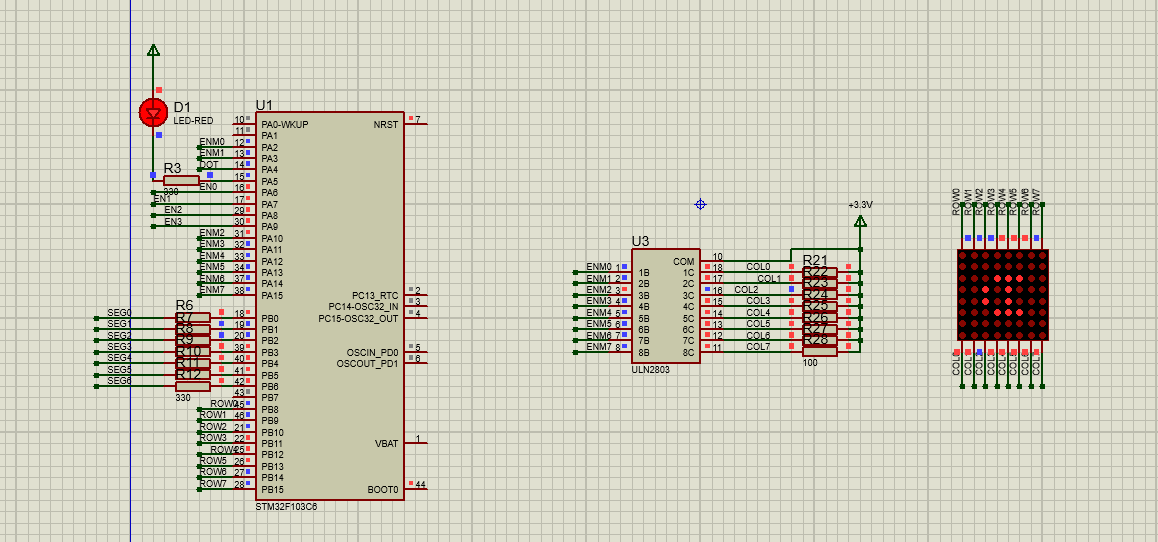
\includegraphics[width=\linewidth]{source/picture/bai_2/lab2_ex9.png}
    \caption{\textit{Proteus schematic for the 8x8 LED matrix in Exercise 9}}
    \label{fig:lab2-ex9-schematic}
\end{figure}

The IOC pin assignment used by the implementation is summarized in
Table~\ref{tab:lab2-ex9-pins}. The eight row pins are contiguous on GPIOB,
while the enable pins use the available GPIOA outputs.

\begin{table}[!htp]
    \centering
    \caption{LED-matrix pin assignment}
    \label{tab:lab2-ex9-pins}
    \begin{tabular}{c|c|l}
        \textbf{Signals} & \textbf{STM32 pins} & \textbf{Function}\\
        \hline
        ENM0--ENM1 & PA2--PA3 & ULN2803 inputs for columns 0--1\\
        ENM2--ENM7 & PA10--PA15 & ULN2803 inputs for columns 2--7\\
        ROW0--ROW7 & PB8--PB15 & Active-high matrix row data\\
    \end{tabular}
\end{table}

\paragraph{Report 2: Matrix buffer and scanning function.}

Each entry in \texttt{matrix\_buffer} contains the eight row states for one
column. Bit 0 controls ROW0 and bit 7 controls ROW7. The following buffer
places a four-by-four letter A in the centre of the display:

\begin{verbatim}
........
........
...##...
..#..#..
..####..
..#..#..
........
........
\end{verbatim}

\begin{lstlisting}[caption={Centered four-by-four letter A stored column-wise}]
const int MAX_LED_MATRIX = 8;
int index_led_matrix = 0;

uint8_t matrix_buffer[8] = {
  0x00U, 0x00U, 0x38U, 0x14U,
  0x14U, 0x38U, 0x00U, 0x00U
};
\end{lstlisting}

The helper function below writes the row byte to PB8--PB15. In
\texttt{updateLEDMatrix()}, all ULN2803 inputs are first driven LOW and the row
outputs are cleared. This blanking interval prevents ghosting while the row
pattern changes. The required row data is then written and exactly one ULN2803
input is driven HIGH to sink the selected column.

\begin{lstlisting}[caption={Row-data output and column scanning for the LED matrix}]
void displayMatrixRows(uint8_t data)
{
  HAL_GPIO_WritePin(ROW0_GPIO_Port, ROW0_Pin,
                    (data & 0x01U) ? GPIO_PIN_SET : GPIO_PIN_RESET);
  HAL_GPIO_WritePin(ROW1_GPIO_Port, ROW1_Pin,
                    (data & 0x02U) ? GPIO_PIN_SET : GPIO_PIN_RESET);
  HAL_GPIO_WritePin(ROW2_GPIO_Port, ROW2_Pin,
                    (data & 0x04U) ? GPIO_PIN_SET : GPIO_PIN_RESET);
  HAL_GPIO_WritePin(ROW3_GPIO_Port, ROW3_Pin,
                    (data & 0x08U) ? GPIO_PIN_SET : GPIO_PIN_RESET);
  HAL_GPIO_WritePin(ROW4_GPIO_Port, ROW4_Pin,
                    (data & 0x10U) ? GPIO_PIN_SET : GPIO_PIN_RESET);
  HAL_GPIO_WritePin(ROW5_GPIO_Port, ROW5_Pin,
                    (data & 0x20U) ? GPIO_PIN_SET : GPIO_PIN_RESET);
  HAL_GPIO_WritePin(ROW6_GPIO_Port, ROW6_Pin,
                    (data & 0x40U) ? GPIO_PIN_SET : GPIO_PIN_RESET);
  HAL_GPIO_WritePin(ROW7_GPIO_Port, ROW7_Pin,
                    (data & 0x80U) ? GPIO_PIN_SET : GPIO_PIN_RESET);
}

void updateLEDMatrix(int index)
{
  HAL_GPIO_WritePin(GPIOA,
                    ENM0_Pin | ENM1_Pin | ENM2_Pin | ENM3_Pin |
                    ENM4_Pin | ENM5_Pin | ENM6_Pin | ENM7_Pin,
                    GPIO_PIN_RESET);
  displayMatrixRows(0x00U);

  if (index < 0 || index >= MAX_LED_MATRIX)
  {
    return;
  }

  displayMatrixRows(matrix_buffer[index]);

  switch (index)
  {
    case 0: HAL_GPIO_WritePin(ENM0_GPIO_Port, ENM0_Pin, GPIO_PIN_SET); break;
    case 1: HAL_GPIO_WritePin(ENM1_GPIO_Port, ENM1_Pin, GPIO_PIN_SET); break;
    case 2: HAL_GPIO_WritePin(ENM2_GPIO_Port, ENM2_Pin, GPIO_PIN_SET); break;
    case 3: HAL_GPIO_WritePin(ENM3_GPIO_Port, ENM3_Pin, GPIO_PIN_SET); break;
    case 4: HAL_GPIO_WritePin(ENM4_GPIO_Port, ENM4_Pin, GPIO_PIN_SET); break;
    case 5: HAL_GPIO_WritePin(ENM5_GPIO_Port, ENM5_Pin, GPIO_PIN_SET); break;
    case 6: HAL_GPIO_WritePin(ENM6_GPIO_Port, ENM6_Pin, GPIO_PIN_SET); break;
    case 7: HAL_GPIO_WritePin(ENM7_GPIO_Port, ENM7_Pin, GPIO_PIN_SET); break;
    default: break;
  }
}
\end{lstlisting}

The matrix scan is executed in \texttt{main()}, as required by the exercise.
TIM2 interrupts every \SI{1}{ms} and only updates the software timers. Whenever
\texttt{timer2\_flag} is raised, the main loop displays the next column and
wraps the index from 7 back to 0.

\begin{lstlisting}[caption={Non-blocking matrix scan in the main loop}]
if (timer2_flag == 1)
{
  setTimer2(1);
  updateLEDMatrix(index_led_matrix);

  index_led_matrix++;
  if (index_led_matrix >= MAX_LED_MATRIX)
  {
    index_led_matrix = 0;
  }
}
\end{lstlisting}

One complete frame requires eight column intervals, so the nominal refresh
frequency is
\[
f_{\mathrm{frame}} = \frac{1}{8\times\SI{1}{ms}} = \SI{125}{Hz}.
\]
This is fast enough for the four-by-four letter A to appear continuously lit
and stationary.

\subsubsection{Exercise 10}

Exercise 10 creates a horizontal animation from the four-by-four letter A in
Exercise 9. The matrix continues to scan one column every \SI{1}{ms}, while a
separate \SI{300}{ms} interval controls the visible movement. Separating these
two time scales keeps the display refresh stable while allowing the character
to move slowly enough to observe.

\paragraph{Report 1: Animation method and source code.}

The animation is implemented by rotating the eight column bytes one position
to the left. The first byte is saved before the shift and written back to the
last position, so pixels leaving the left edge reappear at the right edge. This
cyclic operation produces continuous movement without reconstructing the
letter for every position.

\begin{lstlisting}[caption={Timing state and cyclic left shift for the letter A}]
const uint32_t MATRIX_SHIFT_PERIOD_MS = 300U;
uint32_t matrix_last_shift_tick = 0U;

void shiftMatrixLeft(void)
{
  uint8_t first_column = matrix_buffer[0];

  for (int column = 0; column < (MAX_LED_MATRIX - 1); column++)
  {
    matrix_buffer[column] = matrix_buffer[column + 1];
  }

  matrix_buffer[MAX_LED_MATRIX - 1] = first_column;
}
\end{lstlisting}

Before entering the main loop, the matrix scan timer and animation timestamp
are initialized independently:

\begin{lstlisting}[caption={Initialization of matrix scanning and movement timing}]
setTimer2(1);
matrix_last_shift_tick = HAL_GetTick();
\end{lstlisting}

The elapsed time is checked only when \texttt{index\_led\_matrix} is zero.
Consequently, \texttt{matrix\_buffer} can change only at the boundary between
two complete frames. All eight columns in one frame therefore come from the
same animation position, preventing a visible torn or distorted character.

\begin{lstlisting}[caption={Frame-synchronized animation in the main loop}]
if (timer2_flag == 1)
{
  setTimer2(1);

  if (index_led_matrix == 0)
  {
    uint32_t now = HAL_GetTick();

    if ((uint32_t)(now - matrix_last_shift_tick) >=
        MATRIX_SHIFT_PERIOD_MS)
    {
      matrix_last_shift_tick = now;
      shiftMatrixLeft();
    }
  }

  updateLEDMatrix(index_led_matrix);

  index_led_matrix++;
  if (index_led_matrix >= MAX_LED_MATRIX)
  {
    index_led_matrix = 0;
  }
}
\end{lstlisting}

The TIM2 callback remains short and only calls \texttt{timer\_run()}. Matrix
refresh, animation, seven-segment scanning, clock updates, and DOT control all
remain in the main loop. The resulting animation shifts the letter one column
to the left every \SI{300}{ms} and wraps it continuously across the display.

The Proteus demonstration confirms that the four-by-four letter A remains
stable during each refresh frame and moves continuously from right to left.
When the character reaches the left boundary, its columns reappear from the
right boundary as intended. The complete simulation is available at:
\begin{center}
    \href{https://github.com/quangnguyencomeng/CO3009-261-CC-2453052/blob/main/Lab/lab_reports/source/vids/lab2_ex10.mp4}{\textbf{Exercise 10 demonstration video}}
\end{center}

\endinput




\subsubsection{Exercise 5}
Implement a digital clock with \textbf{hour} and \textbf {minute} information displayed by 2 seven segment LEDs. The code skeleton in the \textbf{main} function is presented as follows:
\begin{lstlisting}[caption=An example for your source code]
int hour = 15, minute = 8, second = 50;

while(1){
    second++;
    if (second >= 60){
        second = 0;
        minute++;
    }
    if(minute >= 60){
        minute = 0;
        hour++;
    }
    if(hour >=24){
        hour = 0;
    }
    updateClockBuffer();
    HAL_Delay(1000);
}
\end{lstlisting}

The function \textbf{updateClockBuffer} will generate values for the array \textbf{led\_buffer} according to the values of hour and minute. In the case these values are 1 digit number, digit 0 is added. \\

\textbf{Report 1: } Present the source code in the \textbf{updateClockBuffer} function.

\subsubsection{Exercise 6}
The main target from this exercise to reduce the complexity (or reduce code processing) in the timer interrupt. The time consumed in the interrupt can lead to the nested interrupt issue, which can crash the whole system. A simple solution can disable the timer whenever the interrupt occurs, the enable it again. However, the real-time processing is not guaranteed anymore.\\

In this exercise, a software timer is created and its counter is count down every timer interrupt is raised (every 10ms). By using this timer, the \textbf{Hal\_Delay(1000)} in the main function is removed. In a MCU system, non-blocking delay is better than blocking delay. The details to create a software timer are presented bellow. The source code is added to your current program, \textbf{do not delete the source code you have on Exercise 5.}\\

\textbf{Step 1: } Declare variables and functions for a software timer, as following:
\begin{lstlisting}[caption=Software timer based timer interrupt]
/* USER CODE BEGIN 0 */
int timer0_counter = 0;
int timer0_flag = 0;
int TIMER_CYCLE = 10;
void setTimer0(int duration){
	timer0_counter = duration /TIMER_CYCLE;
	timer0_flag = 0;
}
void timer_run(){
	if(timer0_counter > 0){
		timer0_counter--;
		if(timer0_counter == 0) timer0_flag = 1;
	}
}
/* USER CODE END 0 */
\end{lstlisting}

Please change the \textbf{TIMER\_CYCLE} to your timer interrupt period. In the manual code above, it is \textbf{10ms}. \\

\textbf{Step 2: } The \textbf{timer\_run()} is invoked in the timer interrupt as following:

\begin{lstlisting}[caption=Software timer based timer interrupt]
void HAL_TIM_PeriodElapsedCallback(TIM_HandleTypeDef *htim){
	
	timer_run();
	
	//YOUR OTHER CODE
}
\end{lstlisting}

\textbf{Step 3: } Use the timer in the main function by invoked setTimer0 function, then check for its flag (timer0\_flag). An example to blink an LED connected to PA5 using software timer is shown as follows:
\begin{lstlisting}[caption=Software timer is used in main fuction to blink the LED]
setTimer0(1000);
while (1){
    if(timer0_flag == 1){
        HAL_GPIO_TogglePin(LED_RED_GPIO_Port, LED_RED_Pin);
        setTimer0(2000);
    }
}
\end{lstlisting}

\textbf{Report 1: } if in line 1 of the code above is miss, what happens after that and why?\\


\textbf{Report 2: } if in line 1 of the code above is changed to setTimer0(1), what happens after that and why?\\

\textbf{Report 3: } if in line 1 of the code above is changed to setTimer0(10), what is changed compared to 2 first questions and why?\\

\subsubsection{Exercise 7}
Upgrade the source code in Exercise 5 (update values for hour, minute and second) by using the software timer and remove the HAL\_Delay function at the end. Moreover, the DOT (connected to PA4) of the digital clock is also moved to main function. \\

\textbf{Report 1: } Present your source code in the while loop on main function.

\subsubsection{Exercise 8}
Move also the update7SEG() function from the interrupt  timer to the main. Finally, the timer interrupt only used to handle  software timers. All processing (or complex computations) is move to an infinite loop on the main function, optimizing the complexity of the interrupt  handler function.\\

\textbf{Report 1: } Present your source code in the the main function. In the case more extra functions are used (e.g. the second software timer), present them in the report as well.

\subsubsection{Exercise 9}

This is an extra works for this lab. A LED Matrix is added to the system. A reference design is shown in figure bellow:
\begin{figure}[!htp]
    \centering
    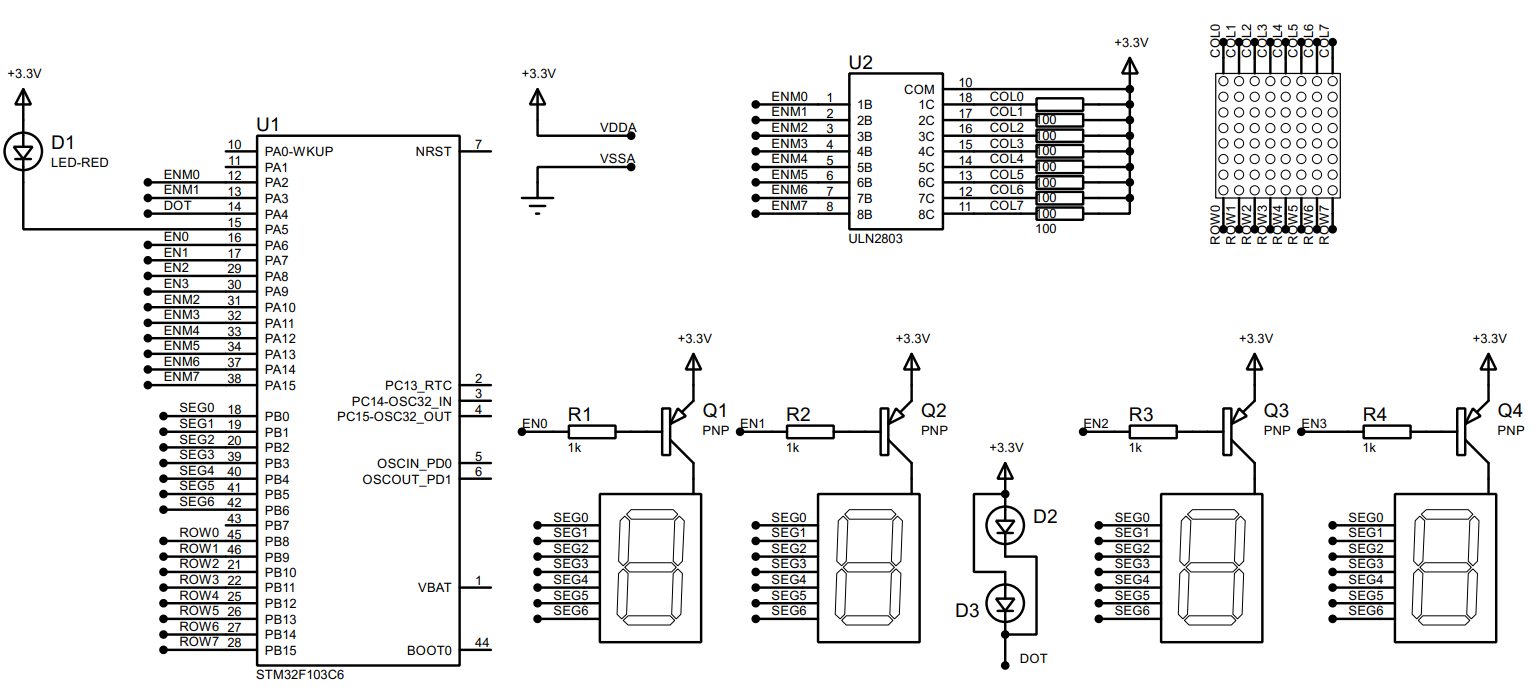
\includegraphics[width=5.5in]{source/picture/bai_2/lab2_m4.PNG}
    \caption{\textit{LED matrix is added to the simulation}}
    \label{bai2_pic9}
\end{figure}

In this schematic, two new components are added, including the \textbf{MATRIX-8X8-RED} and \textbf{ULN2803}, which is an NPN transistor array to enable the power supply for a column of the LED matrix. Students can change the enable signal (from ENM0 to  ENM7) if needed. Finally, the data signal (from ROW0 to ROW7) is connected to PB8 to PB15. \\

\textbf{Report 1: } Present the schematic of your system by capturing the screen in Proteus.\\

\textbf{Report 2: } Implement the function, updateLEDMatrix(int index), which is similarly  to 4 seven led segments.

\begin{lstlisting}[caption=Function to display data on LED Matrix]
const int MAX_LED_MATRIX = 8;
int index_led_matrix = 0;
uint8_t matrix_buffer[8] = {0x01, 0x02, 0x03, 0x04, 0x05, 0x06, 0x07, 0x08};
void updateLEDMatrix(int index){
    switch (index){
        case 0:
            break;
        case 1:
            break;
        case 2:
            break;
        case 3:
            break;
        case 4:
            break;
        case 5:
            break;
        case 6:
            break;
        case 7:
            break;
        default:
            break;
    }
}
\end{lstlisting}

Student are free to choose the invoking frequency of this function. However, this function is supposed to invoked in main function. Finally, please update the \textbf{matrix\_buffer} to display character \textbf{"A"}.

\subsubsection{Exercise 10}
Create an animation on LED matrix, for example, the character is shifted to the left. 

\textbf{Report 1: } Briefly describe your solution and present your source code in the report.
